\documentclass[a4paper,12pt,twoside]{memoir}

% Castellano
\usepackage[spanish,es-tabla]{babel}
\selectlanguage{spanish}
\usepackage[utf8]{inputenc}
\usepackage[T1]{fontenc}
\usepackage{lmodern} % scalable font
\usepackage{microtype}
\usepackage{placeins}

\RequirePackage{booktabs}
\RequirePackage[table]{xcolor}
\RequirePackage{xtab}
\RequirePackage{multirow}

% Links
\PassOptionsToPackage{hyphens}{url}\usepackage[colorlinks]{hyperref}
\hypersetup{
	allcolors = {red}
}

% Acrónimos
\usepackage[acronym]{glossaries}
\makenoidxglossaries

\newacronym{llm}{LLM}{\textit{Large Language Models}}
\newacronym{ods}{ODS}{\textit{Objetivos de Desarrollo Sostenible}}
\newacronym{ods11}{ODS11}{\textit{Ciudades y Comunidades Sostenibles}}
\newacronym{sdg}{SDG}{\textit{Sustainable Development Goals}}
\newacronym{sc}{Smart City}{\textit{Ciudades Inteligentes}}
\newacronym{sdg11}{SDG11}{\textit{Sustainable Cities and Communities}}
\newacronym{poi}{POI}{\textit{Punto de Interés}}
\newacronym{tfg}{TFG}{\textit{Trabajo de Fin de Grado}}


% Ecuaciones
\usepackage{amsmath}

% Rutas de fichero / paquete
\newcommand{\ruta}[1]{{\sffamily #1}}

% Párrafos
\nonzeroparskip

% Huérfanas y viudas
\widowpenalty100000
\clubpenalty100000

% Evitar solapes en el header
\nouppercaseheads

% Imagenes
\usepackage{graphicx}
\newcommand{\imagen}[2]{
	\begin{figure}[!h]
		\centering
		\includegraphics[width=0.9\textwidth]{#1}
		\caption{#2}\label{fig:#1}
	\end{figure}
	\FloatBarrier
}

\newcommand{\imagenflotante}[2]{
	\begin{figure}%[!h]
		\centering
		\includegraphics[width=0.9\textwidth]{#1}
		\caption{#2}\label{fig:#1}
	\end{figure}
}



% El comando \figura nos permite insertar figuras comodamente, y utilizando
% siempre el mismo formato. Los parametros son:
% 1 -> Porcentaje del ancho de página que ocupará la figura (de 0 a 1)
% 2 --> Fichero de la imagen
% 3 --> Texto a pie de imagen
% 4 --> Etiqueta (label) para referencias
% 5 --> Opciones que queramos pasarle al \includegraphics
% 6 --> Opciones de posicionamiento a pasarle a \begin{figure}
\newcommand{\figuraConPosicion}[6]{%
  \setlength{\anchoFloat}{#1\textwidth}%
  \addtolength{\anchoFloat}{-4\fboxsep}%
  \setlength{\anchoFigura}{\anchoFloat}%
  \begin{figure}[#6]
    \begin{center}%
      \Ovalbox{%
        \begin{minipage}{\anchoFloat}%
          \begin{center}%
            \includegraphics[width=\anchoFigura,#5]{#2}%
            \caption{#3}%
            \label{#4}%
          \end{center}%
        \end{minipage}
      }%
    \end{center}%
  \end{figure}%
}

%
% Comando para incluir imágenes en formato apaisado (sin marco).
\newcommand{\figuraApaisadaSinMarco}[5]{%
  \begin{figure}%
    \begin{center}%
    \includegraphics[angle=90,height=#1\textheight,#5]{#2}%
    \caption{#3}%
    \label{#4}%
    \end{center}%
  \end{figure}%
}
% Para las tablas
\newcommand{\otoprule}{\midrule [\heavyrulewidth]}
%
% Nuevo comando para tablas pequeñas (menos de una página).
\newcommand{\tablaSmall}[5]{%
 \begin{table}
  \begin{center}
   \rowcolors {2}{gray!35}{}
   \begin{tabular}{#2}
    \toprule
    #4
    \otoprule
    #5
    \bottomrule
   \end{tabular}
   \caption{#1}
   \label{tabla:#3}
  \end{center}
 \end{table}
}

%
%Para el float H de tablaSmallSinColores
\usepackage{float}

%
% Nuevo comando para tablas pequeñas (menos de una página).
\newcommand{\tablaSmallSinColores}[5]{%
 \begin{table}[H]
  \begin{center}
   \begin{tabular}{#2}
    \toprule
    #4
    \otoprule
    #5
    \bottomrule
   \end{tabular}
   \caption{#1}
   \label{tabla:#3}
  \end{center}
 \end{table}
}

\newcommand{\tablaApaisadaSmall}[5]{%
\begin{landscape}
  \begin{table}
   \begin{center}
    \rowcolors {2}{gray!35}{}
    \begin{tabular}{#2}
     \toprule
     #4
     \otoprule
     #5
     \bottomrule
    \end{tabular}
    \caption{#1}
    \label{tabla:#3}
   \end{center}
  \end{table}
\end{landscape}
}

%
% Nuevo comando para tablas grandes con cabecera y filas alternas coloreadas en gris.
\newcommand{\tabla}[6]{%
  \begin{center}
    \tablefirsthead{
      \toprule
      #5
      \otoprule
    }
    \tablehead{
      \multicolumn{#3}{l}{\small\sl continúa desde la página anterior}\\
      \toprule
      #5
      \otoprule
    }
    \tabletail{
      \hline
      \multicolumn{#3}{r}{\small\sl continúa en la página siguiente}\\
    }
    \tablelasttail{
      \hline
    }
    \bottomcaption{#1}
    \rowcolors {2}{gray!35}{}
    \begin{xtabular}{#2}
      #6
      \bottomrule
    \end{xtabular}
    \label{tabla:#4}
  \end{center}
}

%
% Nuevo comando para tablas grandes con cabecera.
\newcommand{\tablaSinColores}[6]{%
  \begin{center}
    \tablefirsthead{
      \toprule
      #5
      \otoprule
    }
    \tablehead{
      \multicolumn{#3}{l}{\small\sl continúa desde la página anterior}\\
      \toprule
      #5
      \otoprule
    }
    \tabletail{
      \hline
      \multicolumn{#3}{r}{\small\sl continúa en la página siguiente}\\
    }
    \tablelasttail{
      \hline
    }
    \bottomcaption{#1}
    \begin{xtabular}{#2}
      #6
      \bottomrule
    \end{xtabular}
    \label{tabla:#4}
  \end{center}
}

%
% Nuevo comando para tablas grandes sin cabecera.
\newcommand{\tablaSinCabecera}[5]{%
  \begin{center}
    \tablefirsthead{
      \toprule
    }
    \tablehead{
      \multicolumn{#3}{l}{\small\sl continúa desde la página anterior}\\
      \hline
    }
    \tabletail{
      \hline
      \multicolumn{#3}{r}{\small\sl continúa en la página siguiente}\\
    }
    \tablelasttail{
      \hline
    }
    \bottomcaption{#1}
  \begin{xtabular}{#2}
    #5
   \bottomrule
  \end{xtabular}
  \label{tabla:#4}
  \end{center}
}



\definecolor{cgoLight}{HTML}{EEEEEE}
\definecolor{cgoExtralight}{HTML}{FFFFFF}

%
% Nuevo comando para tablas grandes sin cabecera.
\newcommand{\tablaSinCabeceraConBandas}[5]{%
  \begin{center}
    \tablefirsthead{
      \toprule
    }
    \tablehead{
      \multicolumn{#3}{l}{\small\sl continúa desde la página anterior}\\
      \hline
    }
    \tabletail{
      \hline
      \multicolumn{#3}{r}{\small\sl continúa en la página siguiente}\\
    }
    \tablelasttail{
      \hline
    }
    \bottomcaption{#1}
    \rowcolors[]{1}{cgoExtralight}{cgoLight}

  \begin{xtabular}{#2}
    #5
   \bottomrule
  \end{xtabular}
  \label{tabla:#4}
  \end{center}
}




\graphicspath{ {./img/} }

% Capítulos
\chapterstyle{bianchi}
\newcommand{\capitulo}[2]{
	\setcounter{chapter}{#1}
	\setcounter{section}{0}
	\setcounter{figure}{0}
	\setcounter{table}{0}
	\chapter*{#2}
	\addcontentsline{toc}{chapter}{#2}
	\markboth{#2}{#2}
}

% Apéndices
\renewcommand{\appendixname}{Apéndice}
\renewcommand*\cftappendixname{\appendixname}

\newcommand{\apendice}[1]{
	%\renewcommand{\thechapter}{A}
	\chapter{#1}
}

\renewcommand*\cftappendixname{\appendixname\ }

% Formato de portada
\makeatletter
\usepackage{xcolor}
\newcommand{\tutor}[1]{\def\@tutor{#1}}
\newcommand{\course}[1]{\def\@course{#1}}
\definecolor{cpardoBox}{HTML}{E6E6FF}
\def\maketitle{
  \null
  \thispagestyle{empty}
  % Cabecera ----------------
\noindent
\includegraphics[width=\textwidth]{cabecera}\vspace{1cm}%
  \vfill
  % Título proyecto y escudo informática ----------------
  \colorbox{cpardoBox}{%
    \begin{minipage}{.8\textwidth}
      \vspace{.5cm}\Large
      \begin{center}
      \textbf{TFG del Grado en Ingeniería Informática}\vspace{.6cm}\\
      \textbf{\LARGE\@title{}}
      \end{center}
      \vspace{.2cm}
    \end{minipage}

  }%
  \hfill\begin{minipage}{.20\textwidth}
    
\includegraphics[width=\textwidth]{escudoInfor}
  \end{minipage}
  \vfill
  % Datos de alumno, curso y tutores ------------------
  \begin{center}%
  {%
    \noindent\LARGE
    Presentado por \@author{}\\ 
    en Universidad de Burgos --- \@date{}\\
    Tutor: \@tutor{}\\
  }%
  \end{center}%
  \null
  \cleardoublepage
  }
\makeatother


% Datos de portada
\title{Aplicación móvil para la generación de rutas turísticas sostenibles propuestas por modelos de lenguaje de gran escala \\Documentación Técnica}
\author{Fernando Pisot Serrano}
\tutor{Carlos López Nozal}
\date{\today}

\begin{document}

\maketitle



\cleardoublepage


%%%%%%%%%%%%%%%%%%%%%%%%%%%%%%%%%%%%%%%%%%%%%%%%%%%%%%%%%%%%%%%%%%%%%%%%%%%%%%%%%%%%%%%%



\frontmatter


\clearpage

% Indices
\tableofcontents

\clearpage

\listoffigures

\clearpage

\listoftables

\clearpage

\mainmatter

\appendix

\apendice{Plan de Proyecto Software}

\section{Introducción}
El Plan de Proyecto Software es el documento clave que dirige el proceso de desarrollo de la aplicación móvil creada. Este apéndice tiene como objetivo detallar los aspectos críticos de la planificación y gestión del proyecto, asegurando una implementación eficiente y efectiva.
La planificación temporal del proyecto se ha llevado a cabo con el \emph{uso de la metodología ágil} buscando dividir el desarollo en tareas, sprints e hitos que producen un resultado iterativos y bien estructurado, lo que conlleva a una mayor flexibilidad y a la adaptación más efectiva frente los cambios. 

A continuación, se determinará la viabilidad, que reflejará los \emph{recursos humanos y materiales}, así como los costes asociados necesarios para su valoración. La viabilidad incluirá una estimación de los fondos que se basarán en el salario de un trabajador de la imaginación, así como un análisis de los posibles riesgos y su mitigación. Los aspectos económicos y técnicos de la viabilidad son fundamentales, ya que de ellos depende de que el proyecto esté en los límites establecidos y cumpla con los objetivos propuestos.

Este plan es esencial para la gestión del proyecto ya que sirve como una guía detallada, ayudando así a identificar y mitigar riesgos así como a la utilización eficaz de los recursos. Con el enfoque estructurado y ágil, proporcionado por este plan, el equipo de desarrollo podría entregar un producto de alta calidad que, además, cumplirá con el nivel de satisfacción alcanzado entre los usuarios o clientes. 
\section{Planificación temporal}
 Como se ha mencionado anteriormente, la planificación temporal del proyecto se ha llevado a cabo con el uso de metodología ágil: se basa en la división del desarrollo en tareas, sprints e hitos que producen un resultado iterativo y bien estructurado. Esto conlleva una mayor flexibilidad y a la adaptación más efectiva frente a los cambios.

 Algunas herramientas utilizadas para la planificación temporal han sido GitHub y Zube. Ésta última ha permitido la organización de las tareas en tableros Kanban. El uso de GitHub ha permitido gestionar un control de versiones.

 A continuación veremos como la planificación temporal se ha llevado a cabo en diferentes sprints, cómo se ha ido iterando en las diferentes partes del proyecto y cómo se han ido cumpliendo los hitos propuestos. Para ello se mostrarán diferentes diagramas basadas en métricas ágiles.

 Cada tarea se ha dividido en diferentes historias de usuario, que se han ido completando en cada sprint. Cada sprint ha tenido una duración de una o dos semanas, y se han ido completando las tareas propuestas en cada uno de ellos.
 Un ejemplo se puede observar en la siguiente figura ~\ref{fig:issue12}
 \imagen{issue12}{Tarea 12 mostrada en GitHub con la descripción, hito y etiquetas de la tarea a realizar.}

Gracias al uso de la herramienta Zube, se ha podido llevar un control de las tareas a realizar, las tareas completadas y las tareas pendientes. Además, se ha podido llevar un control de los hitos propuestos y de las historias de usuario completadas en cada sprint. Un ejemplo de ello se puede observar en la siguiente figura ~\ref{fig:sprint1}
\imagen{sprint1}{Tablero Kanban de Zube con la gestión de tareas del Sprint 1.}

\subsection{\textit{Hitos}}
Los hitos o milestones son puntos de referencia que marcan el final de un conjunto de tareas. En este proyecto se han definido los siguientes hitos:

\begin{itemize}

    \item \textbf{Kick-off} Puesta en marcha del proyecto. A partir de las reuniones mantenidas con el tutor, se necesita tener todas las herramientas preparadas para empezar a desarrollar tanto la aplicación como su documentación.
    
    \item \textbf{MPV - Mínimo Producto Viable} Se define el MVP como una aplicación móvil que sobre un mapa OSM muestre la ubicación de usuario, obtenga unos POI básicos y una ruta que las una.

    \item \textbf{Checkpoint 1 de documentación} Este milestone agrupa las tareas relacionadas con la creación y actualización de la documentación del proyecto hasta la reunión con el tutor el 1 de septiembre de 2024.

    El objetivo es tener una documentación suficiente para que el tutor pueda dar feedback acerca de la misma y poder corregir errores.

    \item \textbf{Prototipo Prompting} Este prototipo se puede realizar en un cuaderno Jupyter y su objetivo es mostrar la evolución en el prompt que dará como resultado unos POI de mayor calidad.
\end{itemize}

\subsection{Organización en \textit{Sprints}}

Al comenzar este proyecto durante periodo no lectivo se realizaron los Sprint con variación de tiempo de una o dos semanas en función de la planificación personal. Una vez comenzado el curso y con la ayuda del tutor se realizaron reuniones que han servido para, siguiendo la metodología \textit{Agile}, revisar el Sprint anterior, planificar el siguiente y hacer una pequeña retrospectiva para mejorar el trabajo conjunto.


\begin{itemize}
    \item \textbf{Sprint Kick-off(22/07/2024 - 29/07/2024):} Después de las reuniones con el tutor, se establecen los objetivos del proyecto y se comienza a trabajar en la puesta en marcha del proyecto. Se establecen las herramientas a utilizar y se comienza a trabajar en la documentación del proyecto. 33 puntos de historia en 5 tareas.
    ~\ref{fig:bd-kick-off sprint}
\imagen{bd-kick-off sprint}{Figura burndown del Sprint Kick-off.}
    

    \item \textbf{Sprint 1(29/07/2024 - 05/08/2024):} Con las herramientas y una idea previa establecida, es el momento de empezar a desarrollar.

    Objetivos: seguir formándome en LLM y las opciones que pueda implementar en el prototipo de prompt.
    Empezar a desarrollar la aplicación móvil con las características básicas.
    Aprender a documentar sprints, indicar elementos que tendré que documentar y aquellos que tenga claro ir documentando para hacer un avance significativo que pueda evaluar mi tutor.
    
    \item \textbf{Sprint 2(05/08/2024 - 12/08/2024):} A partir del concepto básico, se añaden pequeñas mejoras en los tres aspectos del proyecto.
    
    Objetivos: mejorar el prototipo de prompting del cuaderno Jupyter hasta incorporar un sistema RAG, incluir marcadores al mapa en cuanto al desarrollo y continuar con la documentación.
    
    \textit{Dificultades encontradas}: la documentación me hizo perder mucho tiempo debido a problemas con las librerías, después de mucho tiempo reinicié el proyecto desde la plantilla dada, insertando el texto, lo que solucionó el problema. En cuanto al diseño de la aplicación, el desarrollo fue lento al tener que evaluar diferentes opciones ya que la mayoría de fuentes utilizan mapas de Google, opción que se quería descartar.

    \item \textbf{Sprint 3(12/08/2024 - 22/08/2024):} Este sprint fue más largo que los anteriores para mejorar el resultado final ya que la intención era dejar el proyecto en un estado de revisión lo más completo posible para afrontar la reunión prevista para inicio de septiembre con el tutor del mismo. Al intentar desarrollar la tecnología de enrutado del usuario se comprendió lo que ya se intuía en el sprint anterior y es que basar el trabajo en servicios de Google iba a reportar en un desarrollo más fácil y un resultado más robusto y fiable como se justifica en la sección 5 de la memoria de este \acrshort{tfg}.
    
    \item \textbf{Sprint 4(22/08/2024 - 02/09/2024):} El objetivo es mostrar la versión más completa de la aplicación, la documentación y ahondar en el uso de nuevas herramientas como Figma como herramienta de diseño de aplicaciones y LangFlow a la hora de utilizar otro modelo de prototipo.
    
\end{itemize}

\subsection{Métricas Ágiles}

\section{Estudio de viabilidad}

\subsection{Viabilidad económica}

\subsection{Viabilidad legal}



\apendice{Especificación de Requisitos}

\section{Introducción}
En esta sección se presentan los requisitos de la aplicación, abordando tanto los objetivos generales como los específicos del proyecto. Se incluye un catálogo detallado de los requisitos funcionales y no funcionales, que definen el comportamiento y las características técnicas de la aplicación. Además, se proporciona una especificación detallada de los requisitos a través de tablas de casos de uso, complementadas con su respectivo diagrama de casos de uso, lo que facilita una comprensión clara de las interacciones principales de los usuarios con el sistema.


\section{Objetivos generales}
La misión fundamental de este proyecto persigue conseguir los siguientes propósitos:
\begin{itemize}
	\item \textbf{Fomentar el turismo sostenible:} Facilitar a los usuarios la exploración de ciudades promoviendo al mostrar rutas no motorizadas y modos de transporte como caminar y el uso de bicicletas.
	
	\item \textbf{Optimización de experiencias turísticas personalizadas:} Ofrecer a los usuarios rutas personalizadas que se ajusten a sus intereses y preferencias, proporcionando información detallada y relevante sobre los puntos de interés seleccionados.
	
	\item \textbf{Promover el uso de tecnologías inteligentes en el turismo:} Utilizar tecnologías avanzadas como servicios GIS, Google Places y LLM para mejorar la experiencia del usuario, facilitando la generación automática de rutas y la obtención de información actualizada sobre los destinos turísticos.
	
	\item \textbf{Mejorar la accesibilidad a la información turística:} Proporcionar una plataforma fácil de usar que permita a los usuarios acceder rápidamente a descripciones, fotos y otros datos sobre los puntos de interés, mejorando su experiencia de exploración en las ciudades.
	
	\item \textbf{Rutas generadas sin intereses comerciales:} Generar rutas turísticas sin influencias comerciales, ofreciendo una experiencia imparcial y auténtica, en contraste con otras aplicaciones de recomendaciones de viajes.
\end{itemize}

\section{Catálogo de requisitos}
\subsection{Requisitos funcionales}
\begin{itemize}
	\item \textbf{RF-1 Solicitar permisos de uso de GPS:} La aplicación solicitará el permiso para acceder al GPS cuando se inicie por primera vez, ya que es necesario para calcular y mostrar la ubicación del usuario en tiempo real.
	
	\item \textbf{RF-2 Solicitud de activación de GPS:} Si el GPS está desactivado, la aplicación redirigirá a una pantalla que indicará al usuario la necesidad de activarlo para el correcto funcionamiento de la aplicación.
	
	\item \textbf{RF-3 Activación/Desactivación de seguimiento de usuario:} La aplicación mostrará en tiempo real el recorrido del usuario en el mapa, y este seguimiento podrá activarse o desactivarse en cualquier momento mediante un botón.
	
	\item \textbf{RF-4 Centrar la situación actual del usuario sobre el mapa:} El usuario podrá centrar manualmente su posición en el mapa mediante un botón dedicado. Además, existe la opción de fijar la ubicación del usuario en el centro del mapa durante su recorrido.
	
	\item \textbf{RF-5 Selección de Tour:} El usuario rellenará un formulario indicando el lugar que desea visitar, la cantidad de puntos de interés que quiere ver, sus preferencias de transporte (a pie o bicicleta), sus intereses, y el tiempo máximo que quiere dedicar a la ruta.
	
	\item \textbf{RF-6 Cálculo de información a través de un LLM:} La aplicación usará un servicio Gemini para generar los puntos de interés de acuerdo con las preferencias del usuario. Además, un servicio Google Places mejorará los datos proporcionando descripciones, fotos, URL, ratings y número de votos de los \acrshort{pdi}.
	
	\item \textbf{RF-7 Eliminación de \acrshort{pdi}:} El usuario podrá eliminar puntos de interés tanto desde la pantalla del mapa como desde el resumen de la ruta. Cada vez que un \acrshort{pdi} es eliminado o añadido, la ruta se recalcula automáticamente para ofrecer el trayecto más óptimo.
	
	\item \textbf{RF-8 Cálculo de ruta optimizada:} La aplicación calculará la ruta más corta que conecte los puntos de interés seleccionados por el usuario, adaptándose al medio de transporte elegido (a pie o bicicleta).
	
	\item \textbf{RF-9 Capacidad de añadir un \acrshort{pdi}:} El usuario podrá agregar manualmente un lugar introduciendo su nombre en la barra de búsqueda. Si el lugar existe en los servicios de Google, será añadido automáticamente a la ruta; de lo contrario, no se tomará ninguna acción.
	
	\item \textbf{RF-10 Unirse a Eco City Tour:} El usuario podrá unirse a la ruta existente en cualquier momento. La aplicación calculará la ruta más corta para conectarlo con el tour.
	
	\item \textbf{RF-11 Mejora de los puntos de interés con servicio de obtención de información:} Los datos de los puntos de interés se enriquecerán con información adicional obtenida de Google Places, incluyendo ratings, imágenes, URL y número de votos, mejorando la experiencia del usuario.
	
	\item \textbf{RF-12 Guardado y carga de las rutas turísticas:} el usuario podrá guardar los tours que quiera y tendrá acceso a los mismos desde la pantalla de configuración del Eco City Tour.
	
\end{itemize}

\subsection{Requisitos no funcionales}
\begin{itemize}
	\item \textbf{RNF-1 Rendimiento:} la aplicación debe demostrar un tiempo de respuesta aceptable para que su manejo sea fluido y la carga de datos sea razonable al enlazar varios servicios asíncronos, de tal manera que no se perjudique la experiencia de usuario. 
	\item \textbf{RNF-2 Usabilidad:} Eco City Tours debe ser intuitiva y fácil de entender y utilizar.
	\item \textbf{RNF-3 Disponibilidad:} la aplicación debe estar disponible independientemente de la localización del usuario.
	\item \textbf{RNF-4 Mantenibilidad:} la aplicación debe ser fácilmente modificable debido a su carácter modular, facilitando el mantenimiento para el desarrollador. Además, \textbf{el uso de SonarCloud} ayuda a asegurar la calidad del código mediante el análisis continuo, lo que permite identificar y corregir errores potenciales y optimizar el código, favoreciendo así la mantenibilidad a largo plazo.
	
	\item \textbf{RNF-5 Escalabilidad:} Eco City Tours debe ser capaz de gestionar eficientemente un crecimiento continuo en el número de usuarios, adaptándose sin problemas para ofrecer un rendimiento óptimo incluso en situaciones de alta demanda.
	\item \textbf{RNF-6 Soporte:} la aplicación debe funcionar en versiones actuales de Android sin problemas de rendimiento o fallos en alguna de sus funcionalidades
\end{itemize}
\clearpage

\section{Especificación de requisitos}

\subsection{Actores del sistema}

\begin{table}[H]
	\centering
	\begin{tabularx}{\linewidth}{ p{0.21\columnwidth} p{0.71\columnwidth} }
		\toprule
		\textbf{Actor}    & A01 \\
		\toprule
		\textbf{Nombre:} 			  & \textbf{Usuario} \\
		\textbf{Versión}              & 1.0    \\
		\textbf{Autor}                & \autor \\
		\textbf{Descripción}          & Persona que interactúa con la aplicación Eco City Tour para generar y gestionar rutas turísticas personalizadas. \\
		\textbf{Tipo}                 & Usuario \\
		\textbf{Objetivo}             & Generar, visualizar y personalizar rutas turísticas basadas en puntos de interés y preferencias personales. \\
		\textbf{Responsabilidades}    & 
		\begin{itemize}
			\tightlist
			\item Completar el formulario de preferencias para generar una ruta.
			\item Visualizar detalles de puntos de interés.
			\item Añadir o eliminar puntos de interés de la ruta.
			\item Iniciar y detener el seguimiento de ubicación.
		\end{itemize}\\
		\textbf{Relaciones con casos de uso} & CU01(\ref{cu:config-parametros}), CU02.1(\ref{cu:visualizar-detalles}), CU2.2(\ref{cu:eliminar-pdi}), CU04(\ref{cu:guardar-tour}), CU05(\ref{cu:cargar-tour}). \\
		\bottomrule
	\end{tabularx}
	\caption{A01 - Usuario}
	\label{actor:usuario}
\end{table}

\begin{table}[H]
	\centering
	\begin{tabularx}{\linewidth}{ p{0.21\columnwidth} p{0.71\columnwidth} }
		\toprule
		\textbf{Actor}    & A02 \\
		\toprule
		\textbf{Nombre:} 			  & \textbf{Cloud Firestore} \\
		\textbf{Versión}              & 1.0    \\
		\textbf{Autor}                & \autor \\
		\textbf{Descripción}          & Servicio que posibilita el guardado y carga de las rutas obtenidas por la aplicación. \\
		\textbf{Tipo}                 & Sistema \\
		\textbf{Objetivo}             & Guardar y cargar Eco City Tours generados por el Usuario~(\ref{actor:usuario}). \\
		\textbf{Responsabilidades}    & 
		\begin{itemize}
			\tightlist
			\item Guardar ruta generada.
			\item Cargar en el mapa el Eco City Tour guardado en base de datos.
			\item Borrar los Eco City Tour almacenados.
		\end{itemize}\\
		\textbf{Relaciones con casos de uso} & CU04(\ref{cu:guardar-tour}), CU05(\ref{cu:cargar-tour}) \\
		\bottomrule
	\end{tabularx}
	\caption{A02 - Cloud Firestore}
	\label{actor:firestore}
\end{table}


\begin{table}[H]
	\centering

	\begin{tabularx}{\linewidth}{ p{0.21\columnwidth} p{0.71\columnwidth} }
		\toprule
		\textbf{Actor-ID}    & A03 \\
		\toprule
		\textbf{Nombre: } 			  & \textbf{Gemini-pro 1.5} \\
		\textbf{Versión}              & 1.0    \\
		\textbf{Autor}                & \autor \\
		\textbf{Descripción}          & Servicio externo que proporciona una lista de puntos de interés (POI) basados en las preferencias del usuario. \\
		\textbf{Tipo}                 & Sistema \\
		\textbf{Objetivo}             & Suministrar información relevante sobre puntos de interés en función de los criterios del usuario. \\
		\textbf{Responsabilidades}    & 
		\begin{itemize}
			\tightlist
			\item Consultar la información de \acrshort{pdi} según las preferencias de búsqueda del usuario.
			\item Enviar los datos de los \acrfull{pdi} a la aplicación para generar la ruta.
		\end{itemize}\\
		\textbf{Relaciones con casos de uso} & CU01.1(\ref{cu:calcular-tour})\\
		\bottomrule
	\end{tabularx}
	\caption{A03 - Gemini Pro 1.5}
	\label{actor:gemini}
\end{table}

\begin{table}[H]
	\centering

	\begin{tabularx}{\linewidth}{ p{0.21\columnwidth} p{0.71\columnwidth} }
		\toprule
		\textbf{Actor-ID}    & A04 \\
		\toprule
		\textbf{Nombre: } 			  & \textbf{Google Places Service} \\
		\textbf{Versión}              & 1.0    \\
		\textbf{Autor}                & \autor \\
		\textbf{Descripción}          & Servicio externo encargado de mejorar la información sobre los puntos de interés proporcionando detalles adicionales como descripciones, fotos y valoraciones. \\
		\textbf{Tipo}                 & Sistema \\
		\textbf{Objetivo}             & Enriquecer la información de los \acrlong{pdi} para que el usuario obtenga datos detallados y actualizados sobre cada lugar. \\
		\textbf{Responsabilidades}    & 
		\begin{itemize}
			\tightlist
			\item Proveer información detallada sobre los \acrshort{pdi}.
			\item Enviar las descripciones, fotos y valoraciones de los \acrshort{pdi} a la aplicación.
		\end{itemize}\\
		\textbf{Relaciones con casos de uso} & CU01.1 (\ref{cu:calcular-tour})\\
		\bottomrule
	\end{tabularx}
	\caption{A04 - Google Places Service}
	\label{actor:google-places}
\end{table}

\begin{table}[H]
	\centering

	\begin{tabularx}{\linewidth}{ p{0.21\columnwidth} p{0.71\columnwidth} }
		\toprule
		\textbf{Actor-ID}    & A05 \\
		\toprule
		\textbf{Nombre: } 			  & \textbf{Google Direction Service} \\
		\textbf{Versión}              & 1.0    \\
		\textbf{Autor}                & \autor \\
		\textbf{Descripción}          & Servicio externo encargado de generar una ruta actualizada entre los \acrshort{pdi} que componen el Eco City Tour. \\
		\textbf{Tipo}                 & Sistema \\
		\textbf{Objetivo}             & Proveer la mejor ruta a mostrar en el mapa que conecte los \acrshort{pdi} de cada \textit{Eco City Tour} en cada momento. \\
		\textbf{Responsabilidades}    & 
		\begin{itemize}
			\tightlist
			\item Generar el camino que ha de seguir el usuario de manera más corta según el medio de transporte elegido.
			\item Actualizar en cada momento el camino más corto entre los distintos lugares.
		\end{itemize}\\
		\textbf{Relaciones con casos de uso} & CU01.1 (\ref{cu:calcular-tour})CU02 (\ref{cu:navegar-mapa}) \\
		\bottomrule
	\end{tabularx}
	\caption{A05 - Google Direction Service}
	\label{actor:google-directions}
\end{table}

\begin{table}[H]
	\centering
	\begin{tabularx}{\linewidth}{ p{0.21\columnwidth} p{0.71\columnwidth} }
		\toprule
		\textbf{Actor-ID}    & A06 \\
		\toprule
		\textbf{Nombre: }			  & \textbf{Crashlytics} \\
		\textbf{Versión}              & 1.0    \\
		\textbf{Autor}                & \autor \\
		\textbf{Descripción}          & Servicio externo encargado de registrar en todo momento si se produce un error en la ejecución de la aplicación. \\
		\textbf{Tipo}                 & Sistema \\
		\textbf{Objetivo}             & Dejar constancia en un log de los errores que se puedan llevar a cabo en la ejecución. \\
		\textbf{Responsabilidades}    & 
		\begin{itemize}
			\tightlist
			\item Detectar errores fatales en la ejecución de la aplicación.
			\item Registrar en la nube los detalles que formaron la excepción, para posterior análisis.
		\end{itemize}\\
		\textbf{Relaciones con casos de uso} & CU06 (\ref{cu:registro-log}) \\
		\bottomrule
	\end{tabularx}
	\caption{A06 - Crashlytics}
		\label{actor:crashlytics}
\end{table}
\subsection{Casos de uso}
\label{subsec:casos-uso}
\subsection{CU00 - Configuración GPS}
\begin{figure}[H]
	\centering
	\includegraphics[scale=0.6]{CU00-Gestión-de-GPS}
	\caption{Diagrama de caso de uso CU00 - Configuración GPS}
	\label{fig:CU00-Gestión-de-GPS}
\end{figure}

Este caso de uso es fundamental, ya que sin el permiso de GPS o la activación del sensor, el resto de funcionalidades de la aplicación no pueden ejecutarse. Para mayor claridad y facilitar la lectura de los diagramas restantes, se presenta por separado, destacando su papel como requisito previo para las demás operaciones.

\begin{table}[H]
	\centering
	\begin{tabularx}{\linewidth}{ p{0.21\columnwidth} p{0.71\columnwidth} }
		\toprule
		\textbf{CU00}    & \textbf{Configuración GPS} \\
		\toprule
		\textbf{Versión}              & 1.0    \\
		\textbf{Actor}                & A01 Usuario (\ref{actor:usuario}) \\
		\textbf{Autor}                & \autor \\
		\textbf{Requisitos asociados} & RF-1, RF-2 \\
		\textbf{Descripción}          & Configura la aplicación para tener acceso a la ubicación mediante GPS. \\
		\textbf{Precondición}         & La aplicación está instalada y abierta por primera vez o tras haber revocado permisos anteriormente. \\
		\textbf{Acciones}             &
		\begin{enumerate}
			\def\labelenumi{\arabic{enumi}.}
			\tightlist
			\item La aplicación solicita permiso para el uso del GPS.
			\item El usuario concede el permiso.
			\item La aplicación detecta si el GPS está activado.
			\item Si el GPS no está activado, solicita al usuario activarlo.
		\end{enumerate}\\
		\textbf{Postcondición}        & La aplicación tiene acceso a la ubicación en tiempo real. \\
		\textbf{Excepciones}          & 
		\begin{itemize}
			\tightlist
			\item El usuario no concede el permiso de GPS.
			\item El usuario no activa el GPS cuando se le solicita.
		\end{itemize}\\
		\textbf{Importancia}          & Alta \\
		\textbf{Casos de Prueba}      & 
		\begin{itemize}
			\tightlist
			\item \textbf{Prueba 1 - Permiso concedido:} La aplicación solicita y obtiene acceso al GPS cuando el usuario concede el permiso.\vspace{2pt}
			\item \textbf{Prueba 2 - Permiso denegado:} El usuario deniega el permiso. La aplicación no avanza al mapa y no permite operar sobre la aplicación. \vspace{2pt}
			\item \textbf{Prueba 3 - GPS desactivado:} El GPS está apagado. La aplicación solicita activación y detecta si el usuario lo enciende.
		\end{itemize}\\
		\bottomrule
	\end{tabularx}
	\caption{CU00 Configuración GPS}
\end{table}



\subsection{Casos de uso general}

\begin{figure}[H]
	\centering
	\hspace*{-2cm}
	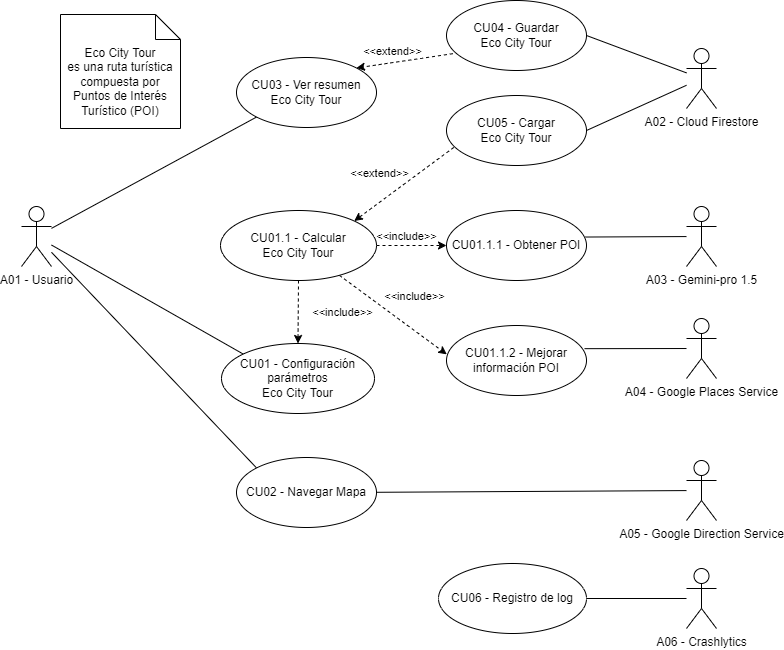
\includegraphics[scale=0.6]{casos-de-uso}
	\caption{Diagrama de casos de uso general de Eco City Tours}
	\label{fig:casos-de-uso}
\end{figure}

\subsection{CU01 - Configuración de parámetros Eco City Tour}

\begin{table}[H]
	\centering
	\begin{tabularx}{\linewidth}{ p{0.21\columnwidth} p{0.71\columnwidth} }
		\toprule
		\textbf{CU01}    & \textbf{Configuración parámetros Eco City Tour} \\
		\toprule
		\textbf{Versión}              & 1.0    \\
		\textbf{Actor}                & A01 Usuario (\ref{actor:usuario}) \\
		\textbf{Autor}                & \autor \\
		\textbf{Requisitos asociados} & RF-5 \\
		\textbf{Descripción}          & Configurar los parámetros necesarios para generar un Eco City Tour personalizado según las preferencias del usuario. \\
		\textbf{Precondición}         & El usuario accede a la pantalla de configuración. \\
		\textbf{Acciones}             &
		\begin{enumerate}
			\def\labelenumi{\arabic{enumi}.}
			\tightlist
			\item El usuario completa el formulario de preferencias, incluyendo el lugar, número de \acrshort{pdi}, medio de transporte y tiempo máximo.
		\end{enumerate}\\
		\textbf{Postcondición}        & Los parámetros quedan configurados y listos para generar la ruta. \\
		\textbf{Excepciones}          & 
		\begin{itemize}
			\tightlist
			\item El usuario no completa el formulario de configuración.
			\item Error en la carga de los datos de configuración.
		\end{itemize}\\
		\textbf{Importancia}          & Alta \\
		\textbf{Casos de Prueba}      &
		\begin{itemize}
			\item \textbf{Prueba 1 - Configuración correcta:} El usuario completa el formulario correctamente con todos los campos requeridos. El sistema guarda los parámetros y los muestra confirmados en el log del modo debug.
			\vspace{2pt}
			\item \textbf{Prueba 2 - Campos vacíos:} El usuario deja el formulario sin modificar. El sistema muestra un \textit{Eco City Tour} en la mejor ciudad del mundo: Salamanca.
			\vspace{2pt}
			\item \textbf{Prueba 3 - Valores límites:} El usuario introduce valores límite en los campos. El sistema valida los parámetros y los procesa correctamente.
		\end{itemize} \\
		\bottomrule
	\end{tabularx}
	\caption{CU01 Configuración parámetros Eco City Tour}
	\label{cu:config-parametros}
\end{table}


\subsection{CU01.1 - Calcular Eco City Tour}

\begin{table}[H]
	\centering
	\begin{tabularx}{\linewidth}{ p{0.21\columnwidth} p{0.71\columnwidth} }
		\toprule
		\textbf{CU01.1}    & \textbf{Calcular Eco City Tour} \\
		\toprule
		\textbf{Versión}              & 1.0    \\
		\textbf{Actor}                & A03 (\ref{actor:gemini}), A04 (\ref{actor:google-places}), A05 (\ref{actor:google-directions}) \\
		\textbf{Autor}                & \autor \\
		\textbf{Requisitos asociados} & RF-6, RF-8 \\
		\textbf{Descripción}          & Generar una ruta optimizada conectando los puntos de interés seleccionados en función de las preferencias del usuario. \\
		\textbf{Precondición}         & Los parámetros han sido configurados correctamente. \\
		\textbf{Acciones}             &
		\begin{enumerate}
			\def\labelenumi{\arabic{enumi}.}
			\tightlist
			\item El usuario confirma la configuración de preferencias.
			\item El sistema consulta un LLM para obtener \acrshort{pdi} basados en las preferencias del usuario.
			\item El sistema envía los \acrshort{pdi} a Google Places para obtener información mejorada.
			\item El sistema consulta un servicio de optimización de rutas para generar la ruta optimizada.
		\end{enumerate}\\
		\textbf{Postcondición}        & La ruta optimizada es calculada y lista para ser visualizada. \\
		\textbf{Excepciones}          & 
		\begin{itemize}
			\tightlist
			\item Fallo en la conexión con el LLM.
			\item Error en el servicio de optimización de rutas.
		\end{itemize}\\
		\textbf{Importancia}          & Alta \\
		\textbf{Casos de Prueba}      &
		\begin{itemize}
			\item \textbf{Prueba 1 - Configuración correcta:} El usuario confirma los parámetros correctamente. El sistema calcula la ruta sin errores y muestra los \acrlong{pdi} optimizados.
			\vspace{2pt}
			\item \textbf{Prueba 2 - Fallo en el LLM:} El sistema no obtiene respuesta del LLM. Se muestra un mensaje de error y se sugiere reintentar la consulta.
			\vspace{2pt}
			\item \textbf{Prueba 3 - Servicio de rutas inalcanzable:} El sistema no puede conectarse al servicio de optimización de rutas (Google Directions). El sistema notifica el fallo al usuario y permite volver a intentarlo.
			\vspace{2pt}
			\item \textbf{Prueba 4 - Valores límite en parámetros:} El usuario configura un número mínimo y máximo de \acrshort{pdi}. El sistema muestra correctamente estos valores calculando la ruta.
		\end{itemize} \\
		\bottomrule
	\end{tabularx}
	\caption{CU01.1 Calcular Eco City Tour}
	\label{cu:calcular-tour}
\end{table}


\subsection{CU02 - Navegar Mapa}


\begin{table}[H]
	\centering
	\begin{tabularx}{\linewidth}{ p{0.21\columnwidth} p{0.71\columnwidth} }
		\toprule
		\textbf{CU02}    & \textbf{Navegar Mapa} \\
		\toprule
		\textbf{Versión}              & 1.0    \\
		\textbf{Autor}                & \autor \\
		\textbf{Actor}                & A01 Usuario (\ref{actor:usuario}) \\
		\textbf{Requisitos asociados} & RF-4 \\
		\textbf{Descripción}          & El usuario puede desplazarse y explorar el mapa interactivo de la aplicación. \\
		\textbf{Precondición}         & El mapa está visible. \\
		\textbf{Acciones}             &
		\begin{enumerate}
			\def\labelenumi{\arabic{enumi}.}
			\tightlist
			\item El usuario explora el mapa desplazándose y haciendo zoom.
		\end{enumerate}\\
		\textbf{Postcondición}        & El usuario navega por el mapa para observar los \acrshort{pdi} y la ruta. \\
		\textbf{Importancia}          & Media \\
		\textbf{Casos de Prueba}      &
		\begin{itemize}
			\item \textbf{Prueba 1 - Desplazamiento funcional:} El usuario desplaza el mapa arrastrando la pantalla con un gesto táctil. El sistema responde correctamente mostrando las áreas correspondientes sin retraso injustificado.
			\vspace{2pt}
			\item \textbf{Prueba 2 - Zoom funcional:} El usuario realiza gestos de zoom in y zoom out en el mapa. El sistema aumenta y reduce el nivel de zoom de manera fluida.
			\vspace{2pt}
			\item \textbf{Prueba 3 - Carga de marcadores (\acrshort{pdi}):} Al navegar, los puntos de interés (\acrshort{pdi}) se cargan dinámicamente y son visibles sin retrasos en la interfaz.
			\vspace{2pt}
			\item \textbf{Prueba 4 - Valores límites de zoom:} El sistema limita correctamente el nivel de zoom máximo y mínimo, evitando desplazamientos inválidos.
		\end{itemize} \\
		\bottomrule
	\end{tabularx}
	\caption{CU02 Navegar Mapa}
	\label{cu:navegar-mapa}
\end{table}



\begin{figure}[H]
	\centering
	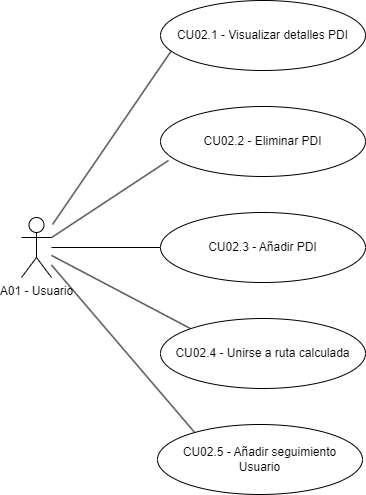
\includegraphics[scale=0.6]{CU02-Navegar-mapa}
	\caption{Diagrama de caso de uso CU02 - Navegar Mapa}
	\label{CU02-Navegar-mapa}
\end{figure}



\begin{table}[H]
	\centering
	\begin{tabularx}{\linewidth}{ p{0.21\columnwidth} p{0.71\columnwidth} }
		\toprule
		\textbf{CU02.1}    & \textbf{Visualizar detalles de \acrfull{pdi}} \\
		\toprule
		\textbf{Versión}              & 1.0    \\
		\textbf{Actor}                & A01 Usuario (\ref{actor:usuario}) \\
		\textbf{Autor}                & \autor \\
		\textbf{Requisitos asociados} & RF-6, RF-11 \\
		\textbf{Descripción}          & El usuario puede obtener información detallada sobre un punto de interés seleccionado en el mapa. \\
		\textbf{Precondición}         & La ruta y los puntos de interés están visibles en el mapa. \\
		\textbf{Acciones}             &
		\begin{enumerate}
			\def\labelenumi{\arabic{enumi}.}
			\tightlist
			\item El usuario selecciona un marcador de punto de interés en el mapa.
			\item El sistema muestra la información detallada del punto de interés.
		\end{enumerate}\\
		\textbf{Postcondición}        & La información detallada del punto de interés es visible para el usuario. \\
		\textbf{Excepciones}          & 
		\begin{itemize}
			\tightlist
			\item Fallo en la carga de información del \acrlong{pdi} debido a problemas de conectividad.
			\item Error en el servicio externo de obtención de información.
		\end{itemize}\\
		\textbf{Importancia}          & Alta \\
		\textbf{Casos de Prueba}      &
		\begin{itemize}
			\item \textbf{Prueba 1 - Información accesible:} El usuario selecciona un marcador de \acrshort{pdi} en el mapa. El sistema carga y muestra correctamente el nombre, descripción, imagen y detalles del \acrlong{pdi}.
			\vspace{2pt}
			\item \textbf{Prueba 2 - Punto sin detalles:} El marcador seleccionado corresponde a un \acrshort{pdi} que no tiene información asociada. El sistema muestra la imagen por defecto y el texto en blanco.
		\end{itemize} \\
		\bottomrule
	\end{tabularx}
	\caption{CU02.1 Visualizar detalles de los \acrfull{pdi}}
	\label{cu:visualizar-detalles}
\end{table}


\begin{table}[H]
	\centering
	\begin{tabularx}{\linewidth}{ p{0.21\columnwidth} p{0.71\columnwidth} }
		\toprule
		\textbf{CU02.2}    & \textbf{Eliminar \acrlong{pdi}} \\
		\toprule
		\textbf{Versión}              & 1.0    \\
		\textbf{Actor}                & A01 (\ref{actor:usuario}), A05 (\ref{actor:google-directions}) \\
		\textbf{Autor}                & \autor \\
		\textbf{Requisitos asociados} & RF-7, RF-8 \\
		\textbf{Descripción}          & El usuario puede eliminar puntos de interés de la ruta desde el mapa. \\
		\textbf{Precondición}         & La ruta ha sido generada y los puntos de interés están visibles en el mapa. \\
		\textbf{Acciones}             &
		\begin{enumerate}
			\def\labelenumi{\arabic{enumi}.}
			\tightlist
			\item El usuario selecciona un punto de interés en el mapa.
			\item El sistema elimina el punto de interés de la ruta.
			\item El sistema recalcula la ruta optimizada sin el punto eliminado.
		\end{enumerate}\\
		\textbf{Postcondición}        & La ruta es recalculada sin el punto de interés eliminado. \\
		\textbf{Excepciones}          & 
		\begin{itemize}
			\tightlist
			\item Error en el recálculo de la ruta.
			\item Problemas de conectividad al intentar actualizar la ruta.
		\end{itemize}\\
		\textbf{Importancia}          & Media \\
		\textbf{Casos de Prueba}      &
		\begin{itemize}
			\item \textbf{Prueba 1 - Eliminación exitosa:} El usuario selecciona un \acrshort{pdi} y el sistema lo elimina correctamente de la ruta. El recálculo de la ruta es exitoso.
			\vspace{2pt}
			\item \textbf{Prueba 2 - Error en el recálculo:} El sistema no logra recalcular la ruta después de la eliminación del \acrshort{pdi}. Se muestra un mensaje de error y la ruta previa se mantiene visible.
			\vspace{2pt}
		\end{itemize} \\
		\bottomrule
	\end{tabularx}
	\caption{CU02.2 Eliminar \acrlong{pdi}}
	\label{cu:eliminar-pdi}
\end{table}


\begin{table}[H]
	\centering
	\begin{tabularx}{\linewidth}{ p{0.21\columnwidth} p{0.71\columnwidth} }
		\toprule
		\textbf{CU02.3}    & \textbf{Añadir \acrfull{pdi}} \\
		\toprule
		\textbf{Versión}              & 1.0    \\
		\textbf{Actor}                & A01 Usuario \ref{actor:usuario} \\
		\textbf{Autor}                & \autor \\
		\textbf{Requisitos asociados} & RF-8, RF-9 \\
		\textbf{Descripción}          & El usuario puede añadir manualmente un nuevo \acrshort{pdi} a la ruta introduciendo su nombre en la barra de búsqueda. \\
		\textbf{Precondición}         & La ruta ha sido generada previamente. \\
		\textbf{Acciones}             &
		\begin{enumerate}
			\def\labelenumi{\arabic{enumi}.}
			\tightlist
			\item El usuario introduce el nombre de un lugar en la barra de búsqueda.
			\item El sistema muestra el resultado de la búsqueda y el usuario lo selecciona para añadirlo.
			\item El sistema recalcula la ruta optimizada incluyendo el nuevo \acrlong{pdi}.
		\end{enumerate}\\
		\textbf{Postcondición}        & El nuevo lugar es añadido a la ruta, y la ruta optimizada es recalculada. \\
		\textbf{Excepciones}          & 
		\begin{itemize}
			\tightlist
			\item El lugar no se encuentra en el servicio de búsqueda.
			\item Fallo en el recalculo de la ruta.
		\end{itemize}\\
		\textbf{Importancia}          & Baja \\
		\textbf{Casos de Prueba}      &
		\begin{itemize}
			\item \textbf{Prueba 1 - Añadir \acrshort{pdi} exitoso:} El usuario introduce el nombre del lugar, el sistema lo encuentra y lo añade correctamente. La ruta es recalculada y optimizada.
			\vspace{2pt}
			\item \textbf{Prueba 2 - Lugar no encontrado:} El usuario introduce un nombre de lugar inexistente. El sistema muestra el listado de lugares vacío pero permite al usuario volver a buscar otro lugar o volver al mapa.
			\vspace{2pt}
			\item \textbf{Prueba 3 - Cálculo de ruta muy larga:} El usuario selecciona un lugar válido, pero no es el que se esperaba al encontrarse muy lejos. El sistema es capaz de ejecutar el cálculo aunque le lleve más tiempo al ser una tarea síncrona. El \acrshort{pdi} se puede eliminar manualmente por el usuario.
		\end{itemize} \\
		\bottomrule
	\end{tabularx}
	\caption{CU02.3 Añadir \acrfull{pdi}}
	\label{cu:añadir-pdi}
\end{table}


\begin{table}[H]
	\centering
	\begin{tabularx}{\linewidth}{ p{0.21\columnwidth} p{0.71\columnwidth} }
		\toprule
		\textbf{CU02.4}    & \textbf{Unirse a la ruta calculada} \\
		\toprule
		\textbf{Versión}              & 1.0    \\
		\textbf{Actor}                & A01 Usuario \ref{actor:usuario} \\
		\textbf{Autor}                & \autor \\
		\textbf{Requisitos asociados} & RF-10 \\
		\textbf{Descripción}          & Permite al usuario unirse a una ruta previamente generada desde su ubicación actual. \\
		\textbf{Precondición}         & Una ruta ya ha sido generada y está activa. \\
		\textbf{Acciones}             &
		\begin{enumerate}
			\def\labelenumi{\arabic{enumi}.}
			\tightlist
			\item El usuario selecciona la opción para unirse a la ruta desde su ubicación actual.
			\item El sistema calcula la ruta más corta para conectar la ubicación actual del usuario con la ruta generada.
		\end{enumerate}\\
		\textbf{Postcondición}        & El usuario es guiado desde su ubicación actual hasta la ruta generada. \\
		\textbf{Excepciones}          & 
		\begin{itemize}
			\tightlist
			\item Error en el cálculo de la ruta de conexión.
		\end{itemize}\\
		\textbf{Importancia}          & Media \\
		\textbf{Casos de Prueba}      &
		\begin{itemize}
			\item \textbf{Prueba 1 - Unirse a la ruta exitosa:} El usuario selecciona la opción para unirse y el sistema calcula correctamente la ruta de conexión.
			\vspace{2pt}
			\item \textbf{Prueba 2 - Ubicación inválida:} El sistema no puede determinar la ubicación actual del usuario. Se muestra la unión al punto más cercano viable del usuario. p.e. si está en mitad del mar lo situaría en la costa.
			\vspace{2pt}
			\item \textbf{Prueba 3 - Ruta previa no generada:} El usuario intenta unirse sin que exista una ruta activa pues es el único punto de la ruta. No se muestra ninguna ruta pero la ubicación formará parte de ella si se añade otra ruta.
			\vspace{2pt}
			\item \textbf{Prueba 4 - Unirse a ruta si está ya unido:} El usuario no puede tener activado el botón de unirse a ruta para evitar el conflicto de unirse múltiples veces.
		\end{itemize} \\
		\bottomrule
	\end{tabularx}
	\caption{CU02.4 Unirse a la ruta calculada}
	\label{cu:unirse-ruta}
\end{table}


\begin{table}[H]
	\centering
	\begin{tabularx}{\linewidth}{ p{0.21\columnwidth} p{0.71\columnwidth} }
		\toprule
		\textbf{CU02.5}    & \textbf{Añadir seguimiento del usuario} \\
		\toprule
		\textbf{Versión}              & 1.0    \\
		\textbf{Actor}                & A01 Usuario (\ref{actor:usuario}) \\
		\textbf{Autor}                & \autor \\
		\textbf{Requisitos asociados} & RF-3 \\
		\textbf{Descripción}          & Permite al usuario activar o desactivar el seguimiento de su posición en tiempo real en el mapa. \\
		\textbf{Precondición}         & La aplicación tiene acceso a la ubicación del usuario. \\
		\textbf{Acciones}             &
		\begin{enumerate}
			\def\labelenumi{\arabic{enumi}.}
			\tightlist
			\item El usuario selecciona la opción de activar o desactivar el seguimiento de su ubicación en el mapa.
			\item El sistema ajusta el mapa para mostrar o dejar de mostrar el movimiento del usuario en tiempo real.
		\end{enumerate}\\
		\textbf{Postcondición}        & El mapa sigue o deja de seguir la posición del usuario en tiempo real. \\
		\textbf{Excepciones}          & 
		\begin{itemize}
			\tightlist
			\item Problemas de conexión con el GPS.
			\item Pérdida de señal GPS.
		\end{itemize}\\
		\textbf{Importancia}          & Baja \\
		\textbf{Casos de Prueba}      &
		\begin{itemize}
			\item \textbf{Prueba 1 - Seguimiento activado:} El usuario activa el seguimiento. El mapa ajusta su vista en tiempo real conforme a la ubicación del usuario.
			\vspace{2pt}
			\item \textbf{Prueba 2 - Seguimiento desactivado:} El usuario desactiva el seguimiento. El mapa deja de ajustarse a la posición del usuario.
			\vspace{2pt}
			\item \textbf{Prueba 3 - Señal GPS débil:} La señal del GPS se pierde temporalmente. El sistema mantendrá la ubicación del usuario en la última ubicación proporcionada (realizado por el Sistema).
		\end{itemize} \\
		\bottomrule
	\end{tabularx}
	\caption{CU02.5 Añadir seguimiento del usuario}
	\label{cu:añadir-seguimiento}
\end{table}



\subsection{CU03 - Ver resumen Eco City Tour}
\begin{table}[H]
	\centering
	\begin{tabularx}{\linewidth}{ p{0.21\columnwidth} p{0.71\columnwidth} }
		\toprule
		\textbf{CU03}    & \textbf{Ver resumen Eco City Tour} \\
		\toprule
		\textbf{Versión}              & 1.0    \\
		\textbf{Actor}                & A01 Usuario \ref{actor:usuario} \\
		\textbf{Autor}                & \autor \\
		\textbf{Requisitos asociados} & RF-4, RF-8 \\
		\textbf{Descripción}          & Muestra un resumen de la ruta generada, incluyendo la distancia, duración y medio de transporte. \\
		\textbf{Precondición}         & La ruta ha sido generada. \\
		\textbf{Acciones}             &
		\begin{enumerate}
			\def\labelenumi{\arabic{enumi}.}
			\tightlist
			\item El usuario accede a la pantalla de resumen.
			\item La aplicación muestra los detalles de la ruta, incluyendo distancia total, tiempo estimado y transporte elegido.
		\end{enumerate}\\
		\textbf{Postcondición}        & El resumen es visible para el usuario. \\
		\textbf{Excepciones}          & 
		\begin{itemize}
			\tightlist
			\item Error en la carga de los datos de la ruta.
		\end{itemize}\\
		\textbf{Importancia}          & Baja \\
		\textbf{Casos de Prueba}      &
		\begin{itemize}
			\item \textbf{Prueba 1 - Resumen completo visible:} El usuario accede a la pantalla de resumen y todos los detalles (distancia, duración y transporte) se muestran correctamente.
			\vspace{2pt}
			\item \textbf{Prueba 2 - Valores límite de distancia y tiempo:} Validar que el sistema maneja correctamente valores grandes (e.g., rutas muy largas) y pequeños (e.g., rutas cortas de menos de 1 km).
			\vspace{2pt}
			\item \textbf{Prueba 3 - Eco City Tour vacío:} Desde la pantalla se eliminan todos los \acrshort{pdi} lo que devuelve al usuario a la pantalla del mapa pues no tiene información útil que mostrar.
		\end{itemize} \\
		\bottomrule
	\end{tabularx}
	\caption{CU03 Ver resumen Eco City Tour}
	\label{cu:resumen}
\end{table}


\subsection{CU04 - Guardar Eco City Tour}
\begin{table}[H]
	\centering
	
	\begin{tabularx}{\linewidth}{ p{0.21\columnwidth} p{0.71\columnwidth} }
		\toprule
		\textbf{CU04}    & \textbf{Guardar Eco City Tour} \\
		\toprule
		\textbf{Versión}              & 1.0    \\
		\textbf{Actor}                & A01~\ref{actor:usuario}, A02~\ref{actor:firestore} \\
		\textbf{Autor}                & \autor \\
		\textbf{Requisitos asociados} & RF-12 \\
		\textbf{Descripción}          & Permite al usuario guardar la ruta generada para acceder a ella en el futuro. \\
		\textbf{Precondición}         & La ruta ha sido generada. \\
		\textbf{Acciones}             &
		\begin{enumerate}
			\def\labelenumi{\arabic{enumi}.}
			\tightlist
			\item El usuario selecciona la opción de guardar la ruta.
		\end{enumerate}\\
		\textbf{Postcondición}        & La ruta queda guardada en el sistema. \\
		\textbf{Excepciones}          & 
		\begin{itemize}
			\tightlist
			\item Error en el guardado de la ruta.
			\item Problemas de conexión con la base de datos.
		\end{itemize}\\
		\textbf{Importancia}          & Media \\
		\textbf{Casos de Prueba}      &
		\begin{itemize}
			\item \textbf{Prueba 1 - Guardado exitoso:} El usuario guarda una ruta y verifica que esta aparece correctamente en el sistema.
			\vspace{2pt}
			\item \textbf{Prueba 2 - Valores límite:} Comprobar el guardado de rutas con diferentes tamaños (e.g., desde una ruta vacía hasta rutas con el número máximo permitido).
			\vspace{2pt}
			\item \textbf{Prueba 3 - Error en la conexión:} Simular la pérdida de conexión (al limitar los permisos de escritura en Firestore) al intentar guardar una ruta y verificar que el sistema muestra un mensaje de error claro sin comprometer la estabilidad.
		\end{itemize} \\
		\bottomrule
	\end{tabularx}
	\caption{CU04 Guardar Eco City Tour}
	\label{cu:guardar-tour}
\end{table}


\subsection{CU05 - Cargar Eco City Tour}
\begin{table}[H]
	\centering
	\begin{tabularx}{\linewidth}{ p{0.21\columnwidth} p{0.71\columnwidth} }
		\toprule
		\textbf{CU05}    & \textbf{Cargar Eco City Tour} \\
		\toprule
		\textbf{Versión}              & 1.0    \\
		\textbf{Actor}                & A01~\ref{actor:usuario}, A02~\ref{actor:firestore} \\
		\textbf{Autor}                & \autor \\
		\textbf{Requisitos asociados} & RF-12 \\
		\textbf{Descripción}          & Permite al usuario cargar una ruta guardada previamente. \\
		\textbf{Precondición}         & El usuario ha guardado al menos una ruta. \\
		\textbf{Acciones}             &
		\begin{enumerate}
			\def\labelenumi{\arabic{enumi}.}
			\tightlist
			\item El usuario selecciona la opción de cargar una ruta guardada.
			\item El usuario selecciona un Eco City Tour guardado previamente que será cargado.
		\end{enumerate}\\
		\textbf{Postcondición}        & La ruta es cargada y visible en el mapa. \\
		\textbf{Excepciones}          & 
		\begin{itemize}
			\tightlist
			\item Error en la carga de la ruta guardada.
			\item Problemas de conexión con la base de datos.
		\end{itemize}\\
		\textbf{Importancia}          & Media \\
		\textbf{Casos de Prueba}      &
		\begin{itemize}
			\item \textbf{Prueba 1 - Carga exitosa:} El usuario selecciona y carga una ruta guardada, verificando que esta aparece correctamente en el mapa.
			\vspace{2pt}
			\item \textbf{Prueba 2 - Valores límite:} Validar la carga de rutas guardadas vacías y rutas con el número máximo de \acrshort{pdi}.
			\vspace{2pt}
			\item \textbf{Prueba 3 - Rutas no existente:} La pantalla de carga solo muestra los Eco City Tour asociados al usuarios y no todos los creados por todos los usuarios y si no tiene ninguno es capaz de mostrar la pantalla vacía con un mensaje amigable.
		\end{itemize} \\
		\bottomrule
	\end{tabularx}
	\caption{CU05 Cargar Eco City Tour}
	\label{cu:cargar-tour}
\end{table}


\subsection{CU06 - Registro de log}
\begin{table}[H]
	\centering
	\begin{tabularx}{\linewidth}{ p{0.21\columnwidth} p{0.71\columnwidth} }
		\toprule
		\textbf{CU06}    & \textbf{Registro de log} \\
		\toprule
		\textbf{Versión}              & 1.0    \\
		\textbf{Actor}                & A06~(\ref{actor:crashlytics}) \\
		\textbf{Autor}                & \autor \\
		\textbf{Descripción}          & Registra los eventos y actividades del usuario en la aplicación para fines de monitorización y depuración. \\
		\textbf{Precondición}         & La aplicación está en funcionamiento. \\
		\textbf{Acciones}             &
		\begin{enumerate}
			\def\labelenumi{\arabic{enumi}.}
			\tightlist
			\item La aplicación registra automáticamente los eventos relevantes.
		\end{enumerate}\\
		\textbf{Postcondición}        & Los eventos quedan registrados en el sistema. \\
		\textbf{Excepciones}          & 
		\begin{itemize}
			\tightlist
			\item Error en la conexión con el sistema de registros.
			\item Fallo en la escritura de los eventos en el log.
		\end{itemize}\\
		\textbf{Importancia}          & Baja \\
		\textbf{Casos de Prueba}      &
		\begin{itemize}
			\item \textbf{Prueba 1 - Registro exitoso:} Verificar que los eventos importantes (inicio de sesión, selección de ruta, activación del GPS) se registran correctamente en el sistema de logs.
			\vspace{2pt}
			\item \textbf{Prueba 2 - Evento límite:} Validar que se registran eventos con mensajes largos o múltiples detalles (e.g., error detallado con trazas largas).
			\vspace{2pt}
			\item \textbf{Prueba 3 - Registro de una caída de la aplicación:} Se puede simular un cierre inesperado que debe ser notificado y visible desde la consola de Crashlytics.
		\end{itemize} \\
		\bottomrule
	\end{tabularx}
	\caption{CU06 Registro de log}
	\label{cu:registro-log}
\end{table}




\apendice{Especificación de diseño}

\section{Introducción}
En este anexo, se detallan las especificaciones de diseño del proyecto, enfocadas en los aspectos fundamentales para el desarrollo de la aplicación. Se describen cómo se organizan los datos que lo componen, el diseño arquitectónico, y los procedimientos empleados. Estas especificaciones son clave para asegurar el correcto funcionamiento y la estructuración adecuada de cada uno de los elementos que componen Eco City Tours.
\section{Diseño de datos}
\imagen{clases}{Diagrama de clases de la aplicación}

\section{Diseño procedimental}

\section{Diseño arquitectónico}
\imagen{components-diagram}{Diagrama de componentes de la aplicación}
\imagen{components-simple}{Diagrama de componentes a nivel de paquetes de la aplicación}
\imagen{secuence}{Diagrama de secuencia - Generación de Eco City Tour}



\apendice{Documentación técnica de programación}

\section{Introducción}
Este anexo proporciona una guía técnica detallada para desarrolladores que deseen trabajar en el proyecto \textbf{Eco City Tours}. Aquí se describe cómo configurar desde el entorno de desarrollo, hasta compilar y ejecutar el proyecto, así como las pruebas realizadas y la configuración de servicios externos necesarios para el correcto funcionamiento de la aplicación. 

\section{Estructura de directorios}
Se ha intentado seguir las buenas prácticas de programación adquiridas en mi formación a la hora de organizar los directorios de la siguiente manera:
\begin{itemize}
	
	\item \textbf{/}: fichero de la licencia, .gitignore y el documento \textit{Readme} con información del proyecto.
	
	\item \textbf{/project-docs/}: documentación del proyecto usando la plantilla \LaTeX  proporcionada.
	
	\item \textbf{/project-prototype/}: dos prototipos de uso de modelos LLM con ejemplos de prompting y técnicas RAG, tanto en un cuaderno Python como en LangFlow así como las conclusiones tras su experimentación.
	
	\item \textbf{/project-app/}: se trata del proyecto Flutter creado a raíz del asistente de Visual Studio y que fue construido de manera incremental desde una aplicación vacía.
	
	
\end{itemize}

\section{Manual del programador}

El objetivo de este manual es servir como referencia para cualquier programador que trabaje en este proyecto. Aquí se detallan los pasos necesarios para configurar el entorno de desarrollo, obtener el código fuente desde el repositorio, compilarlo, ejecutarlo y realizar pruebas. Los pasos son los siguientes:

\subsection{Entorno de desarrollo}

Para trabajar en el desarrollo de \textbf{Eco City Tours}, se recomienda configurar el entorno de desarrollo con las siguientes herramientas:

\begin{itemize}
	\item \textbf{Visual Studio Code:} Editor de código recomendado por su integración con Flutter y extensiones útiles como \texttt{Dart} y \texttt{Flutter}.
	\item \textbf{Android Studio:} Utilizado principalmente para configurar emuladores de dispositivos móviles.
	\item \textbf{Flutter SDK:} Framework utilizado para el desarrollo de aplicaciones multiplataforma. 
	\item \textbf{Copilot:} Extensión para \textit{Visual Studio Code} que utiliza inteligencia artificial para sugerir código y acelerar el desarrollo.
\end{itemize}

\subsubsection{Pasos para configurar el entorno}

\begin{enumerate}
	\item Descarga e instala \textbf{Visual Studio Code} desde \url{https://code.visualstudio.com/}.
	\item Instala las extensiones necesarias para Flutter y Dart:
	\begin{itemize}
		\item Abre la pestaña de extensiones (\texttt{Ctrl+Shift+X}) en Visual Studio Code.
		\item Busca e instala las extensiones \texttt{Flutter} y \texttt{Dart}.
	\end{itemize}
	\item Descarga e instala \textbf{Android Studio} desde \url{https://developer.android.com/studio}.
	\item Configura los emuladores Android en Android Studio:
	\begin{itemize}
		\item Abre el \texttt{AVD Manager}.
		\item Crea un nuevo emulador con las especificaciones necesarias (por ejemplo, Pixel 5 con Android 11 o superior).
	\end{itemize}
	\item Instala el \textbf{Flutter SDK}:
	\begin{itemize}
		\item Descarga el SDK desde su web \cite{flutter_install}
		\item Agrega el binario de Flutter al \texttt{PATH} del sistema:
		\begin{verbatim}
			export PATH="$PATH:/ruta/del/flutter/bin"
		\end{verbatim}
		\item Verifica la instalación ejecutando:
		\begin{verbatim}
			flutter doctor
		\end{verbatim}
		Este comando será muy útil para indicar si falta alguna librería del sistema operativo o indicará si hay problemas pendientes en la configuración.
	\end{itemize}
	\item Instala \textbf{Copilot}:
	\begin{itemize}
		\item Desde la pestaña de extensiones en Visual Studio Code, busca e instala \texttt{GitHub Copilot}.
		\item Inicia sesión con tu cuenta de GitHub para activar la extensión.
	\end{itemize}
\end{enumerate}
El uso de Copilot es gratuito para estudiantes que puedan demostrar su vinculación con una cuenta educativa asociada a GitHub. Durante el proceso de verificación, se solicita capturar dos fotografías a través de una webcam: una que muestre un documento acreditativo, como un carné de estudiante, y otra que incluya una matrícula vigente emitida por la institución educativa correspondiente. Aunque el procedimiento puede parecer sencillo, también es necesario justificar la cercanía geográfica al centro educativo o explicar las razones por las cuales este requisito no se cumple. En el caso de programas de enseñanza online, es posible indicar que, debido a la naturaleza del programa, no es obligatorio residir cerca del centro. Para ello, además de las fotografías requeridas, se puede incluir un archivo PDF que acredite que el grupo de matriculación pertenece a un programa de educación online.

Además de las extensiones necesarias, como \textit{Dart Language} y \textit{Flutter Support}, y de la opcional \textit{GitHub Copilot}, se pueden instalar otras extensiones en Visual Studio Code que dependen de las preferencias y estilo de trabajo de cada programador. A continuación, se presenta una lista de extensiones recomendadas que pueden facilitar y optimizar el desarrollo del proyecto:

\begin{itemize} \item \textbf{Activitus Bar:} Simplifica la navegación entre vistas y herramientas, permitiendo cambiar rápidamente entre el explorador de archivos, la vista de control de versiones y otros paneles de trabajo. \item \textbf{Error Lens:} Muestra los errores y advertencias directamente en el editor, junto al código relevante, para que sean fáciles de identificar y resolver sin necesidad de abrir la consola de problemas. \item \textbf{Paste JSON as Code:} Permite pegar estructuras JSON directamente en el editor y convertirlas automáticamente en modelos o clases de código en lenguaje Dart u otros lenguajes. \item \textbf{Better Comments:} Mejora la legibilidad de los comentarios en el código al aplicar formatos visuales diferenciados, como colores y estilos, para tareas pendientes, advertencias, preguntas o anotaciones importantes. \item \textbf{Pubspec Assist:} Facilita la edición del archivo \texttt{pubspec.yaml} para agregar dependencias de Flutter o Dart sin necesidad de escribirlas manualmente, buscando automáticamente las versiones disponibles. \item \textbf{Bloc:} Ofrece herramientas específicas para desarrollar aplicaciones basadas en el patrón Bloc, ayudando en la organización del código y el manejo del estado. \item \textbf{Awesome Flutter Snippets:} Proporciona fragmentos de código (\textit{snippets}) predefinidos para acelerar la escritura de widgets, estructuras comunes y patrones repetitivos en Flutter. \item \textbf{GitGraph:} Muestra una representación gráfica de las ramas y los \textit{commits} en un repositorio Git, facilitando el seguimiento del historial y la gestión de versiones. \end{itemize}

Estas extensiones no son obligatorias, pero pueden mejorar significativamente la productividad y la experiencia del programador al trabajar en el proyecto \textbf{Eco City Tours}. Su selección dependerá de las necesidades específicas y preferencias de cada desarrollador.

\subsection{Obtención del código fuente}

El código fuente del proyecto está disponible en un repositorio de GitHub. Sigue los pasos a continuación para clonar el repositorio:

\begin{enumerate}
	\item Asegúrate de tener \textbf{Git} instalado en tu sistema. Si no lo tienes, descárgalo e instálalo desde \url{https://git-scm.com/}.
	
	\item Clona el repositorio utilizando el siguiente comando en tu terminal:
	\begin{verbatim}
		git clone https://github.com/fps1001/TFGII_FPisot.git
	\end{verbatim}
	
	\item Cambia al directorio donde se encuentra la aplicación ejecutando:
	\begin{verbatim}
		cd TFGII_FPisot/project-app/project_app
	\end{verbatim}
	
\end{enumerate}




\section{Compilación, instalación y ejecución del proyecto} \label{sec:compilacion}

Esta sección describe los pasos necesarios para compilar, instalar y ejecutar el proyecto \textbf{Eco City Tours}. Incluye la configuración de servicios externos como Google y Firebase, la obtención de claves API y la preparación del entorno de desarrollo.

\subsection{Configuración de Google Cloud Platform}

El proyecto utiliza los siguientes servicios de Google:
\begin{itemize}
	\item \textbf{Google Maps SDK for Android:} Para mostrar mapas en la aplicación.
	\item \textbf{Google Places API:} Para obtener información sobre puntos de interés.
	\item \textbf{Google Directions API:} Para calcular rutas.
	\item \textbf{Generative AI (Gemini):} Para funcionalidades avanzadas basadas en modelos de lenguaje.
\end{itemize}

\subsubsection{Pasos para configurar Google Cloud}
\begin{enumerate}
	\item Regístrate en \href{https://cloud.google.com/}{Google Cloud Platform} y crea un nuevo proyecto.
	\item Activa las siguientes API desde la consola de Google Cloud:
	\begin{itemize}
		\item \texttt{Maps SDK for Android}.
		\item \texttt{Places API}.
		\item \texttt{Directions API}.
		\item \texttt{Generative AI API (Gemini)}.
	\end{itemize}
	\item Genera claves API para cada servicio. Guarda estas claves en un archivo \texttt{.env} ubicado en la raíz del proyecto. El archivo debe tener el siguiente formato:
	\begin{verbatim}
		GOOGLE_API_KEY=<TU_CLAVE>
		GEMINI_API_KEY=<TU_CLAVE>
		GOOGLE_DIRECTIONS_API_KEY=<TU_CLAVE>
		GOOGLE_PLACES_API_KEY=<TU_CLAVE>
	\end{verbatim}
\end{enumerate}

\subsection{Configuración de Firebase}

Firebase se utiliza para almacenamiento en la nube y análisis de errores. Los servicios configurados incluyen:
\begin{itemize}
	\item \textbf{Cloud Firestore:} Base de datos en tiempo real para gestionar datos de la aplicación.
	\item \textbf{Crashlytics:} Herramienta para el análisis y reporte de errores.
\end{itemize}

\subsubsection{Pasos para configurar Firebase}
\begin{enumerate}
	\item Regístrate en \href{https://firebase.google.com/}{Firebase Console} y crea un proyecto con el nombre \texttt{eco-city-tour}.
	\item Configura \textbf{Cloud Firestore}:
	\begin{itemize}
		\item Accede a la consola de Firebase y habilita Firestore en modo "Producción".
	\end{itemize}
	\item Configura \textbf{Crashlytics}:
	\begin{itemize}
		\item Ve a la sección de Crashlytics en Firebase Console y sigue las instrucciones para integrar Crashlytics con tu aplicación.
	\end{itemize}
	\item Descarga el archivo \texttt{google-services.json} desde la consola de Firebase y colócalo en el directorio \texttt{/android/app/} del proyecto.
	\item Agrega las siguientes variables al archivo \texttt{.env}:
	\begin{verbatim}
		FIREBASE_API_KEY=<TU_CLAVE>
		FIREBASE_APP_ID=<TU_CLAVE>
		FIREBASE_MESSAGING_SENDER_ID=<TU_CLAVE>
		FIREBASE_PROJECT_ID=eco-city-tour
		FIREBASE_STORAGE_BUCKET=eco-city-tour.appspot.com
		FIREBASE_PACKAGE_NAME=com.example.project_app
		FIREBASE_PROJECT_NUMBER=<TU_NUMERO>
		MOBILESDK_APP_ID=<TU_CLAVE>
	\end{verbatim}
\end{enumerate}

\subsection{Compilación y ejecución del proyecto}

Una vez configurados los servicios externos, el proyecto puede compilarse y ejecutarse siguiendo estos pasos:
\begin{enumerate}
	\item Asegúrate de que el archivo \texttt{.env} está en la raíz del proyecto.
	\item Instala las dependencias necesarias ejecutando:
	\begin{verbatim}
		flutter pub get
	\end{verbatim}
	\item Compila y ejecuta la aplicación en un dispositivo o emulador:
	\begin{verbatim}
		flutter run
	\end{verbatim}
\end{enumerate}

\section{Pruebas del sistema}

El sistema fue sometido a diversas pruebas para garantizar su correcto funcionamiento, su calidad de código y la cobertura de los casos de uso. A continuación, se detallan los enfoques y herramientas utilizados durante el proceso de pruebas.

\subsection{Control de calidad del código con SonarCloud}

Para evaluar la calidad del código, se utilizó \textbf{SonarCloud}, una herramienta que permite analizar métricas clave como complejidad, mantenibilidad, duplicación de código y cobertura de tests. El análisis de calidad se automatizó a través del flujo de trabajo definido en el archivo \href{https://github.com/fps1001/TFGII_FPisot/tree/main/.github/workflows}{\texttt{.github/workflows}}, donde se configuraron los siguientes pasos:
\begin{itemize}
	\item Ejecución de las pruebas automatizadas para garantizar que no existan errores en el código.
	\item Generación del archivo \texttt{lcov.info}, que contiene los datos de cobertura del proyecto.
	\item Envío automático de la cobertura de código y otros resultados a SonarCloud para su análisis.
\end{itemize}

Este flujo de trabajo se ejecuta automáticamente cada vez que se realiza un \texttt{push} al repositorio o se abre una \texttt{pull request}, permitiendo un control continuo de la calidad del proyecto.


\subsection{Pruebas funcionales y análisis inicial}

Dada la naturaleza del proyecto y el uso de Modelos de Lenguaje de Gran Escala (LLM), inicialmente se realizaron pruebas manuales para evaluar la calidad de los resultados. Estas pruebas se centraron en generar rutas y puntos de interés en la ciudad donde resido, verificando la precisión y relevancia de las recomendaciones generadas.

\subsection{Pruebas automatizadas}

Se implementaron pruebas automatizadas en la carpeta \texttt{test/} del proyecto para garantizar que cada componente funcione correctamente. Las pruebas fueron desarrolladas utilizando los siguientes paquetes de \textbf{Flutter}:

\begin{itemize}
	\item \texttt{test}: Paquete principal para escribir y ejecutar pruebas unitarias.
	\item \texttt{bloc\_test}: Herramienta especializada para probar lógica de negocio implementada con el patrón Bloc.
	\item \texttt{mockito} y \texttt{mocktail}: Utilizados para generar \textit{mocks} de servicios y (\textit{blocs}) según las necesidades de los tests.
\end{itemize}

Cada archivo \texttt{.dart} cuenta con un conjunto de tests que validan su comportamiento esperado. Estos incluyen pruebas unitarias para funciones específicas y pruebas de integración para verificar el correcto flujo entre los componentes.

\subsubsection{Ejecución de los tests}

Para ejecutar las pruebas automatizadas y generar un reporte de cobertura, es necesario ejecutar el siguiente comando en la raíz del proyecto:
\begin{verbatim}
	flutter test --coverage
\end{verbatim}

Este comando ejecuta todos los tests definidos y genera un archivo \texttt{lcov.info} con los datos de cobertura. Estos datos son posteriormente utilizados por SonarCloud para generar un reporte detallado sobre qué partes del código están cubiertas por los tests y cuáles no.
\imagen{sonarcloud}{Resumen de análisis de la rama principal en SonarCloud}
\subsection{Conclusiones de las pruebas}

El sistema fue sometido a un conjunto completo de pruebas funcionales y de calidad, logrando:
\begin{itemize}
	\item Identificar y corregir errores en fases tempranas del desarrollo.
	\item Garantizar una alta cobertura del código, reflejada en los reportes de SonarCloud.
	\item Validar la precisión y relevancia de las recomendaciones generadas por los LLM en contextos reales.
\end{itemize}

Estas pruebas aseguran que el proyecto \textbf{Eco City Tours} cumple con los estándares de calidad necesarios para un entorno de producción.

\apendice{Documentación de usuario}

\section{Introducción}
Esta sección tiene como objetivo proporcionar a los usuarios las instrucciones necesarias para instalar, configurar y utilizar la aplicación Eco City Tours. Este manual está dirigido a usuarios finales interesados en explorar ciudades de manera sostenible, sin necesidad de conocimientos técnicos avanzados.
En primer lugar, se describirán los requisitos mínimos necesarios para ejecutar la aplicación. A continuación, se detallarán los pasos necesarios para instalarla. Finalmente, se presentará una guía práctica para que el usuario pueda aprovechar todas las funcionalidades que ofrece la aplicación.
\section{Requisitos de usuarios}
Para garantizar el correcto funcionamiento de \textbf{Eco City Tours}, el dispositivo debe cumplir con los siguientes requisitos:

\subsection*{Requisitos del Sistema Operativo}
\begin{itemize}
	\item \textbf{Versión mínima de Android:} 6.0 (API 23, Marshmallow).
	\item \textbf{Versión objetivo de Android:} 14 (API 34, Upside Down Cake).
	\item La aplicación está optimizada para las características más recientes de Android 14.
\end{itemize}

\subsection*{Permisos Requeridos}
La aplicación solicita ciertos permisos para ofrecer funcionalidades avanzadas, como el acceso a internet y a la ubicación. Sin embargo, los permisos de localización no son necesarios para iniciar la aplicación y se solicitarán al usuario únicamente cuando sean relevantes para la funcionalidad requerida.

\subsection*{Requisitos de Hardware}
\begin{itemize}
	\item Dispositivo con soporte para \textbf{GPS} y ubicación.
	\item Procesador compatible con arquitecturas ARM o x86.
	\item Acceso a Internet mediante Wi-Fi o red móvil.
\end{itemize}

\section{Instalación}

Para instalar la aplicación \textbf{Eco City Tours} en un dispositivo compatible, siga los siguientes pasos:

\begin{enumerate}
	\item Acceda al repositorio oficial del proyecto en GitHub utilizando el siguiente enlace: 
	\url{https://github.com/fps1001/TFGII_FPisot/releases}.
	\item Busque la \textbf{versión más reciente} de las releases disponibles. Asegúrese de seleccionar la versión adecuada para su dispositivo.
	\item Descargue el archivo \texttt{.apk} correspondiente a esa versión.
	\item Una vez descargado, abra el archivo en su dispositivo móvil para iniciar el proceso de instalación.
	\item Si es la primera vez que instala una aplicación fuera de Google Play Store, es posible que deba habilitar la opción de \textbf{Permitir aplicaciones de fuentes desconocidas} en los ajustes de seguridad de su dispositivo.
	\item Siga las instrucciones que aparecen en pantalla para completar la instalación.
\end{enumerate}

Una vez instalado, la aplicación estará lista para ser configurada y utilizada según las indicaciones del presente manual.

\section{Manual del Usuario}
A continuación, se describen todas las operaciones que puede realizar un usuario de \textbf{Eco City Tours}, explicando todas las funcionalidades de la aplicación, así como los pasos necesarios para utilizarlas de manera efectiva.

\subsection{Habilitar el permiso de uso de GPS}
\begin{figure}[h!]
	\centering
	\begin{tabular}{m{0.4\textwidth} m{0.55\textwidth}}
		
\includegraphics[width=1\linewidth]{E1-habilitar-gps} & 
		\vspace{-10pt}
		
			La primera acción que debe realizar el usuario al iniciar la aplicación es habilitar el permiso de uso de GPS. Esto permite que la aplicación acceda a la ubicación del dispositivo para calcular rutas y mostrar información relevante.
			\textbf{Pasos a seguir:}
			\begin{enumerate}
				\item Al abrir la aplicación por primera vez, aparecerá la pantalla mostrada en la Figura~\ref{fig:habilitarGPS}.
				\item Pulse el botón \textbf{Solicitar acceso al GPS}.
				\item Conceda el permiso solicitado en la ventana emergente.
			\end{enumerate}		
	\end{tabular}
	\caption{Habilitar el permiso de uso de GPS}
	\label{fig:habilitarGPS}
\end{figure}
\newpage
\subsection{Seleccionar opciones de Eco City Tour}
\begin{figure}[h!]
	\centering
	\begin{tabular}{m{0.4\textwidth} m{0.55\textwidth}}
		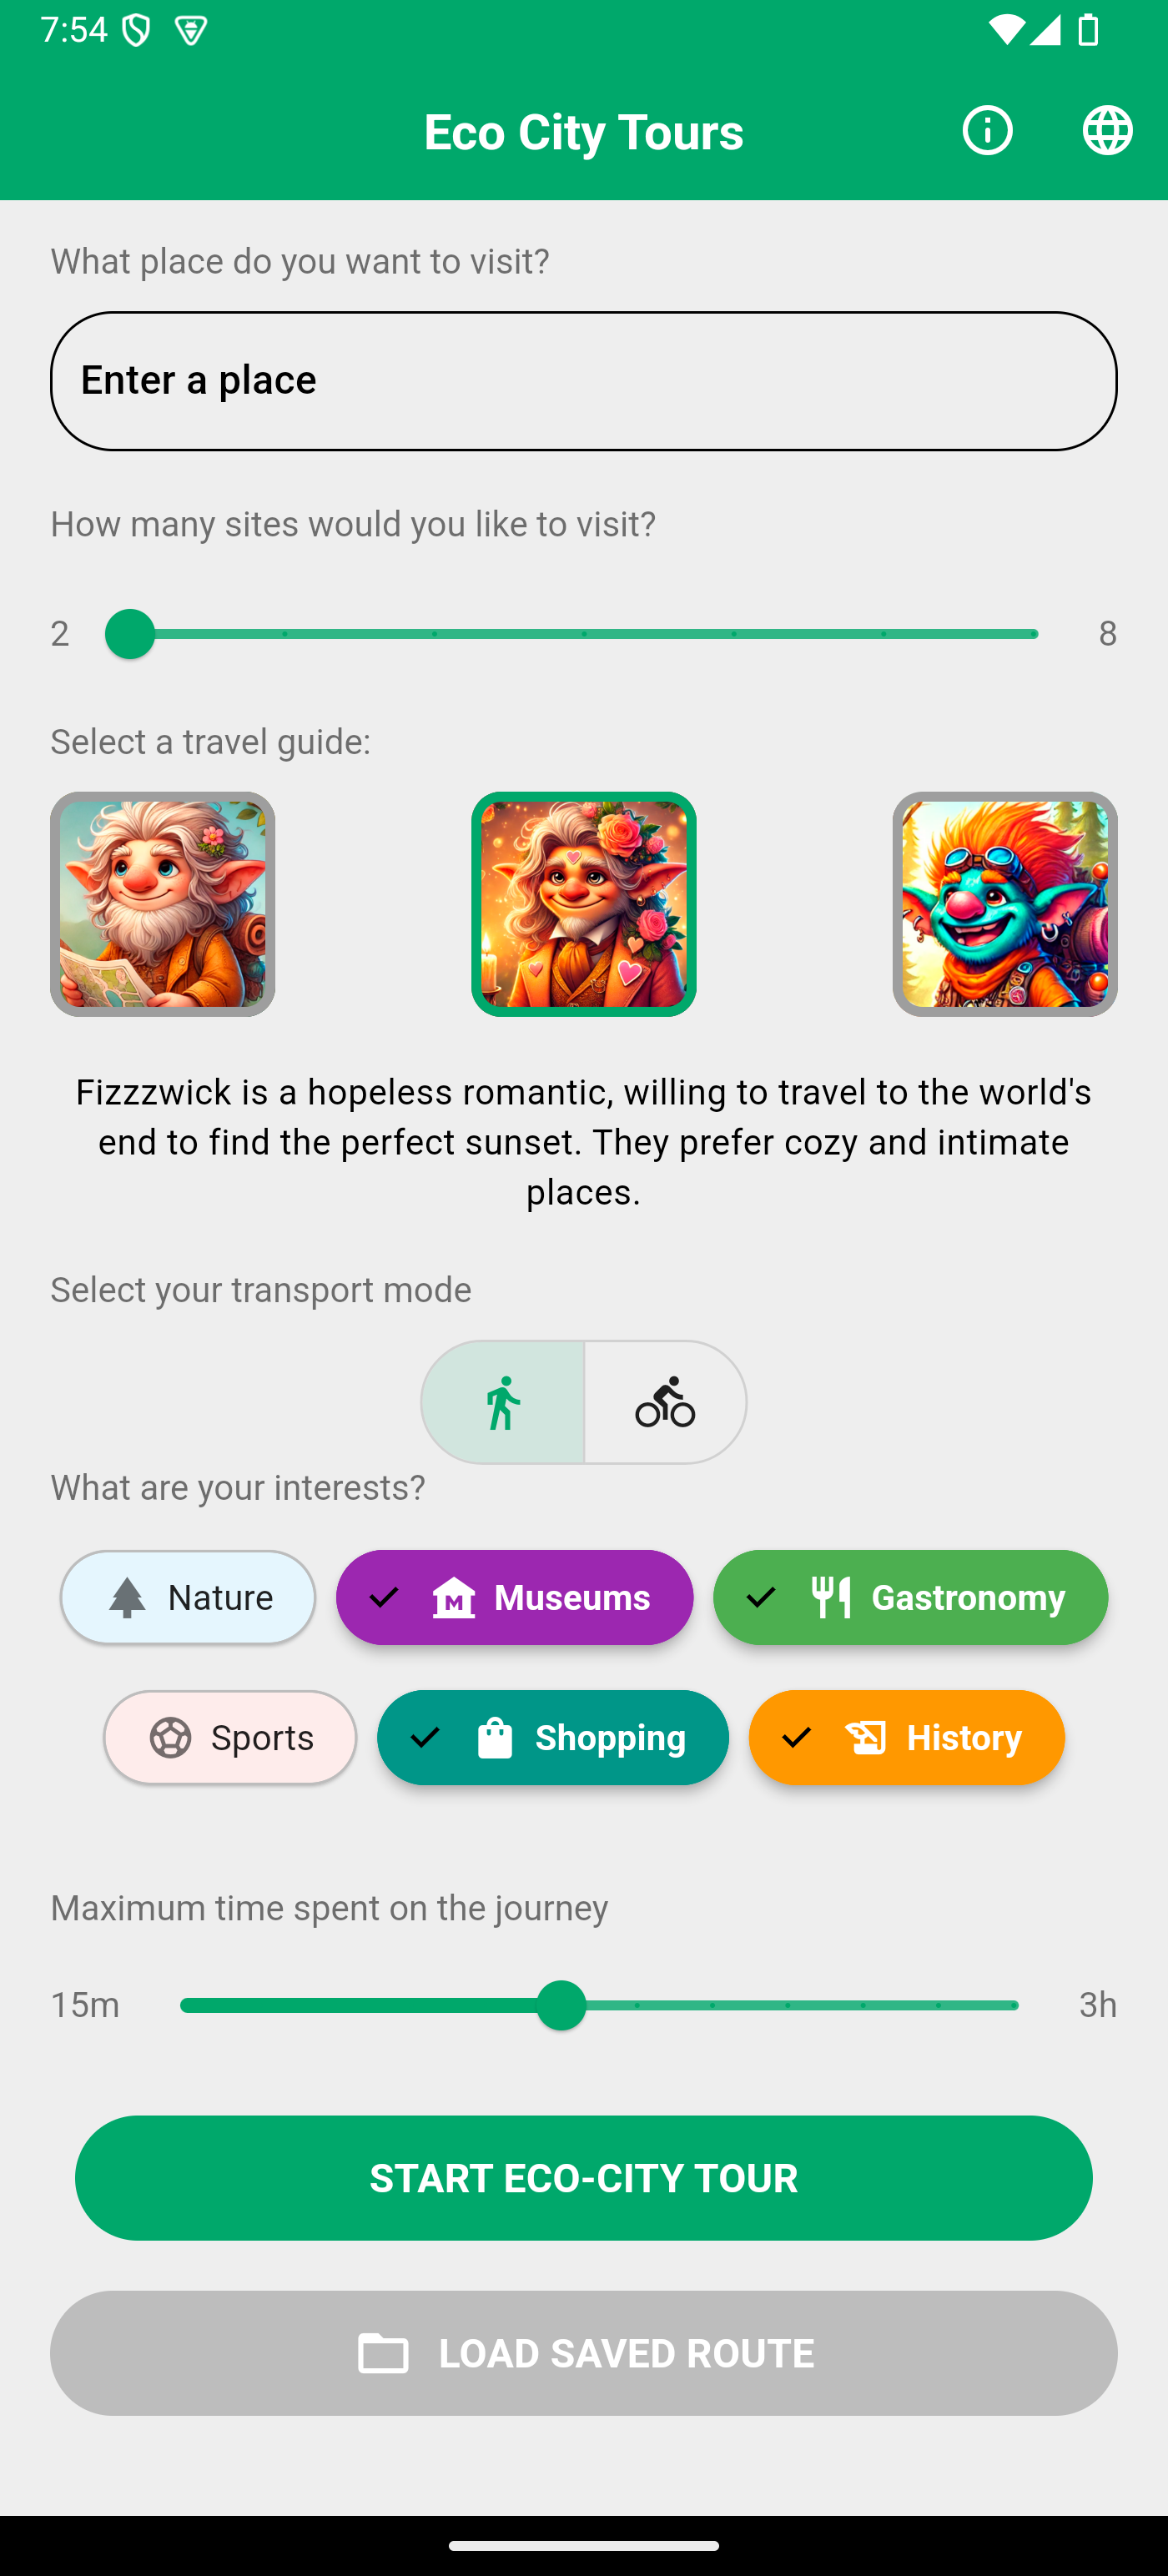
\includegraphics[width=0.6\linewidth]{E2-selection-tour-screen} &		
		
		La primera acción que debe realizar el usuario al iniciar la aplicación es habilitar el permiso de uso de GPS. Esto permite que la aplicación acceda a la ubicación del dispositivo para calcular rutas y mostrar información relevante.
		\textbf{Pasos a seguir:}
		\begin{enumerate}
			\item Al abrir la aplicación por primera vez, aparecerá la pantalla mostrada en la Figura~\ref{fig:selectionTourScreen}.
			\item Pulse el botón \textbf{Solicitar acceso al GPS}.
			\item Conceda el permiso solicitado en la ventana emergente.
		\end{enumerate}		
	\end{tabular}
	\caption{Pantalla de configuración de Eco City Tour}
	\label{fig:selectionTourScreen}
\end{figure}
\subsection{Visualizar Eco City Tour generado}
\begin{figure}[h!]
	\centering
	\begin{tabular}{m{0.4\textwidth} m{0.55\textwidth}}
		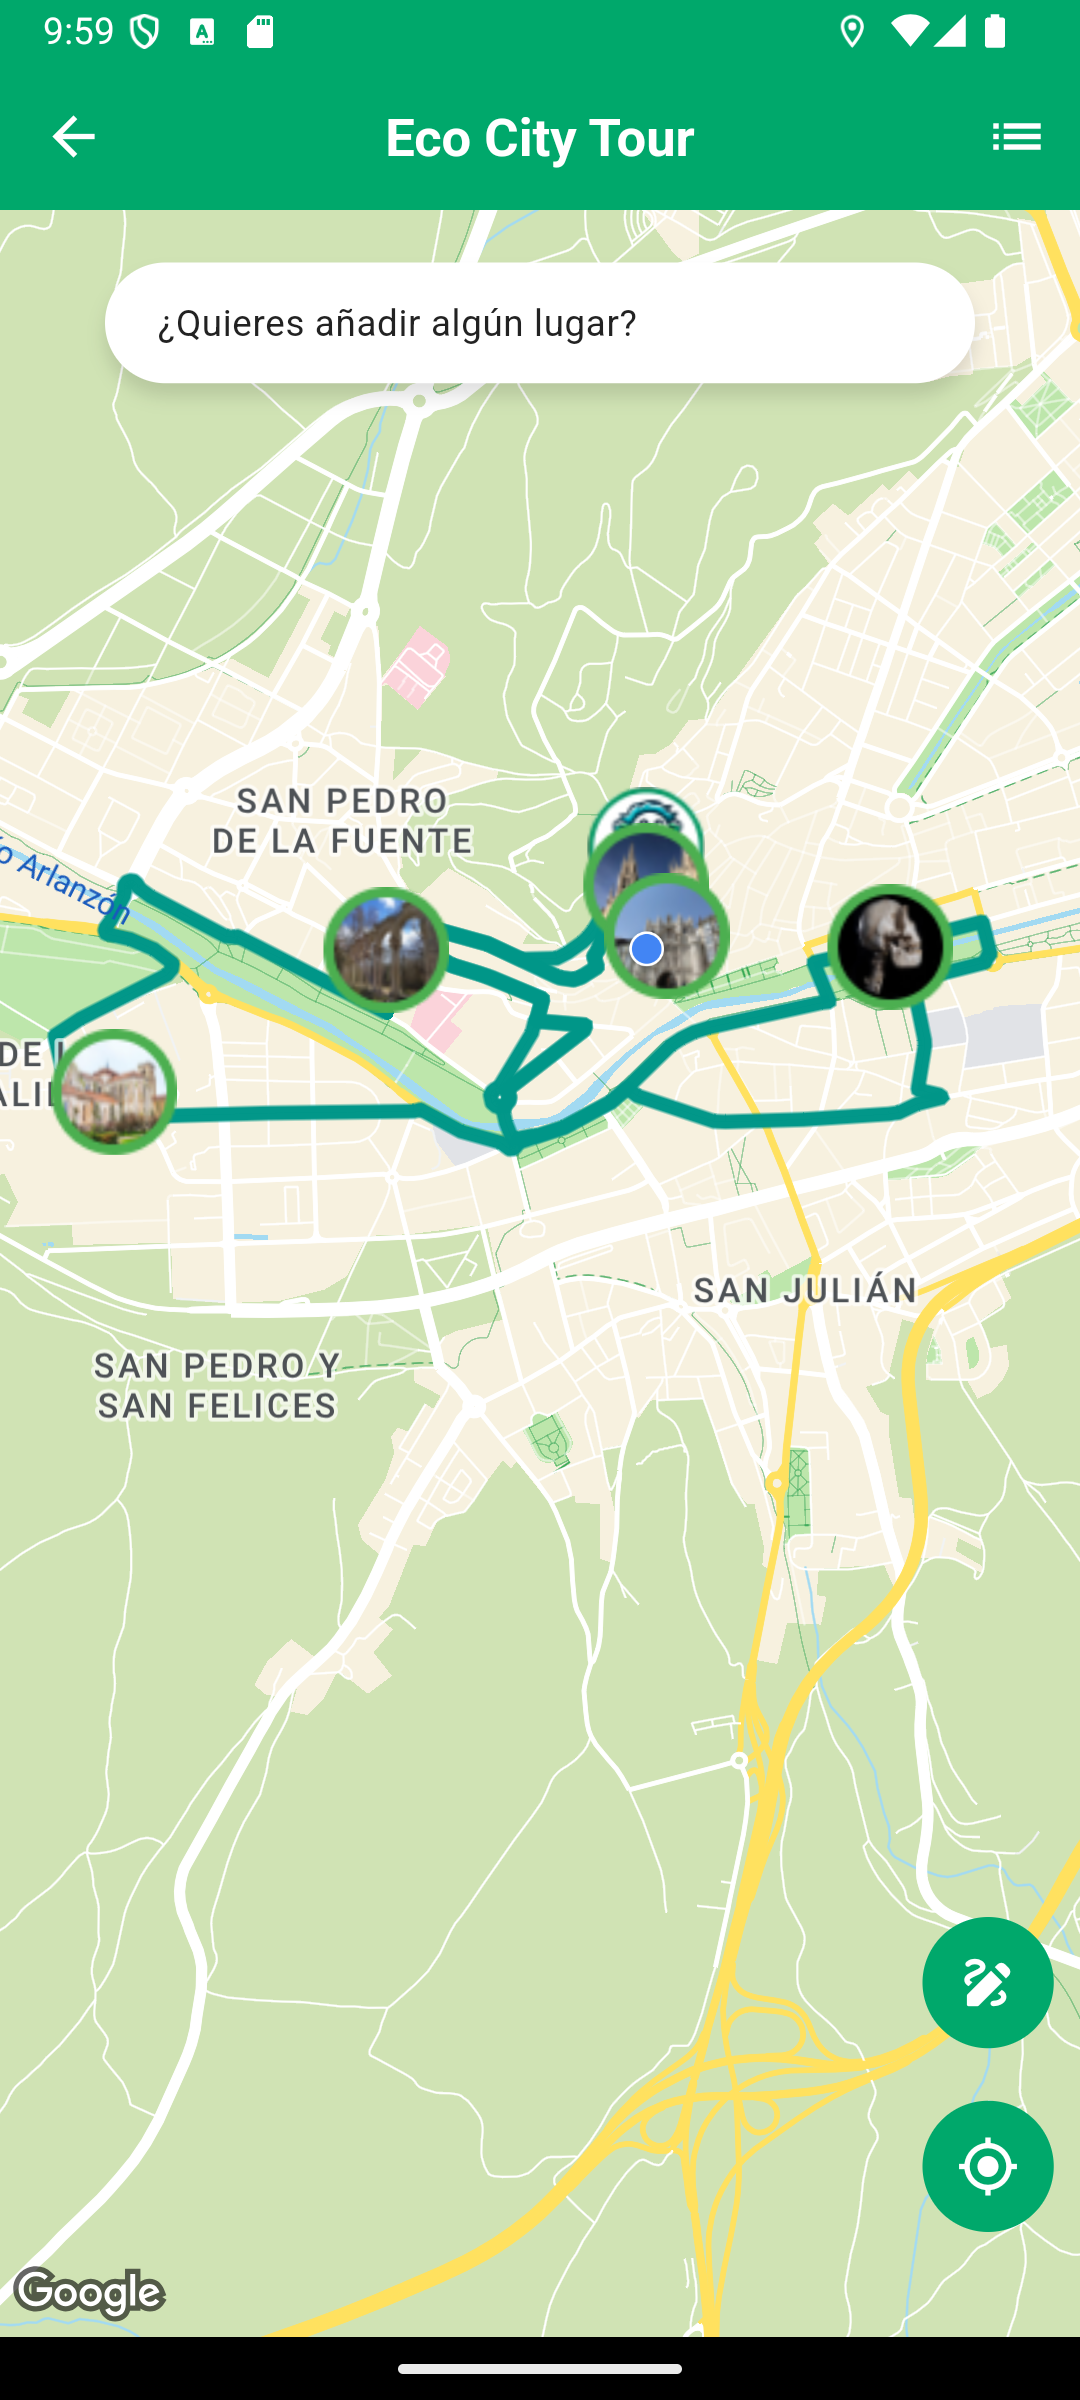
\includegraphics[width=0.6\linewidth]{E3-map-screen} & 
		\vspace{-10pt}
		
		La primera acción que debe realizar el usuario al iniciar la aplicación es habilitar el permiso de uso de GPS. Esto permite que la aplicación acceda a la ubicación del dispositivo para calcular rutas y mostrar información relevante.
		\textbf{Pasos a seguir:}
		\begin{enumerate}
			\item Al abrir la aplicación por primera vez, aparecerá la pantalla mostrada en la .
			\item Pulse el botón \textbf{Solicitar acceso al GPS}.
			\item Conceda el permiso solicitado en la ventana emergente.
		\end{enumerate}		
	\end{tabular}
	\caption{Pantalla de navegación de mapa}
	\label{fig:navegacionMapa}
\end{figure}

\subsection{Buscar y añadir un \acrlong{pdi} al Eco City Tour}
\begin{figure}[h!]
	\centering
	\begin{tabular}{m{0.4\textwidth} m{0.55\textwidth}}
		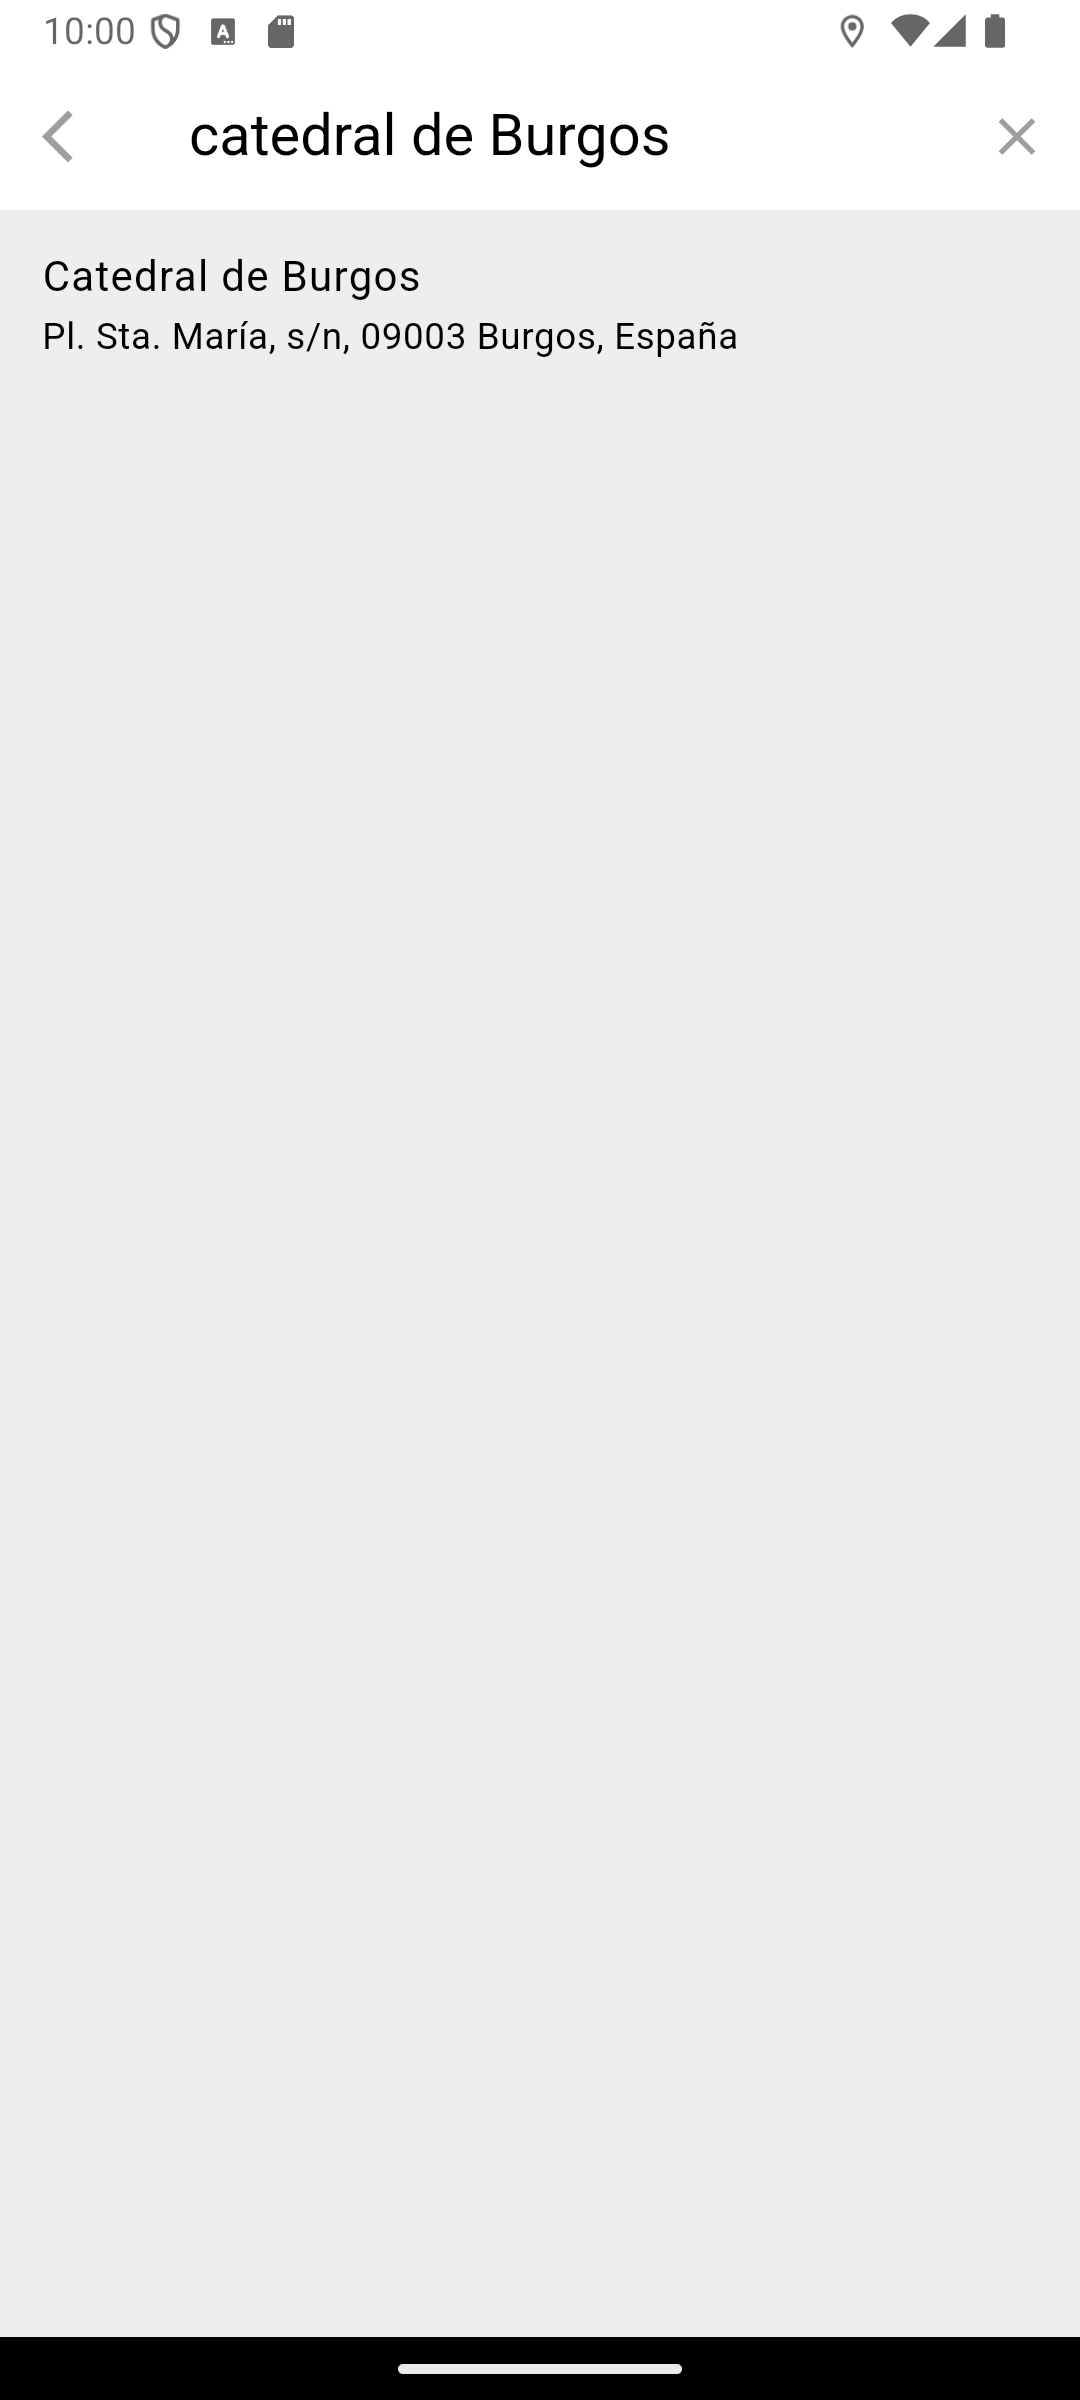
\includegraphics[width=0.6\linewidth]{E4-search-bar} & 
		\vspace{-10pt}
		
		La primera acción que debe realizar el usuario al iniciar la aplicación es habilitar el permiso de uso de GPS. Esto permite que la aplicación acceda a la ubicación del dispositivo para calcular rutas y mostrar información relevante.
		\textbf{Pasos a seguir:}
		\begin{enumerate}
			\item Al abrir la aplicación por primera vez, aparecerá la pantalla mostrada en la Figura~\ref{fig:busquedaPDI}.
			\item Pulse el botón \textbf{Solicitar acceso al GPS}.
			\item Conceda el permiso solicitado en la ventana emergente.
		\end{enumerate}		
	\end{tabular}
	\caption{Búsqueda de \acrshort{pdi}}
	\label{fig:busquedaPDI}
\end{figure}

\subsection{Conocer detalle de \acrshort{pdi}}
\begin{figure}[h!]
	\centering
	\begin{tabular}{m{0.4\textwidth} m{0.55\textwidth}}
		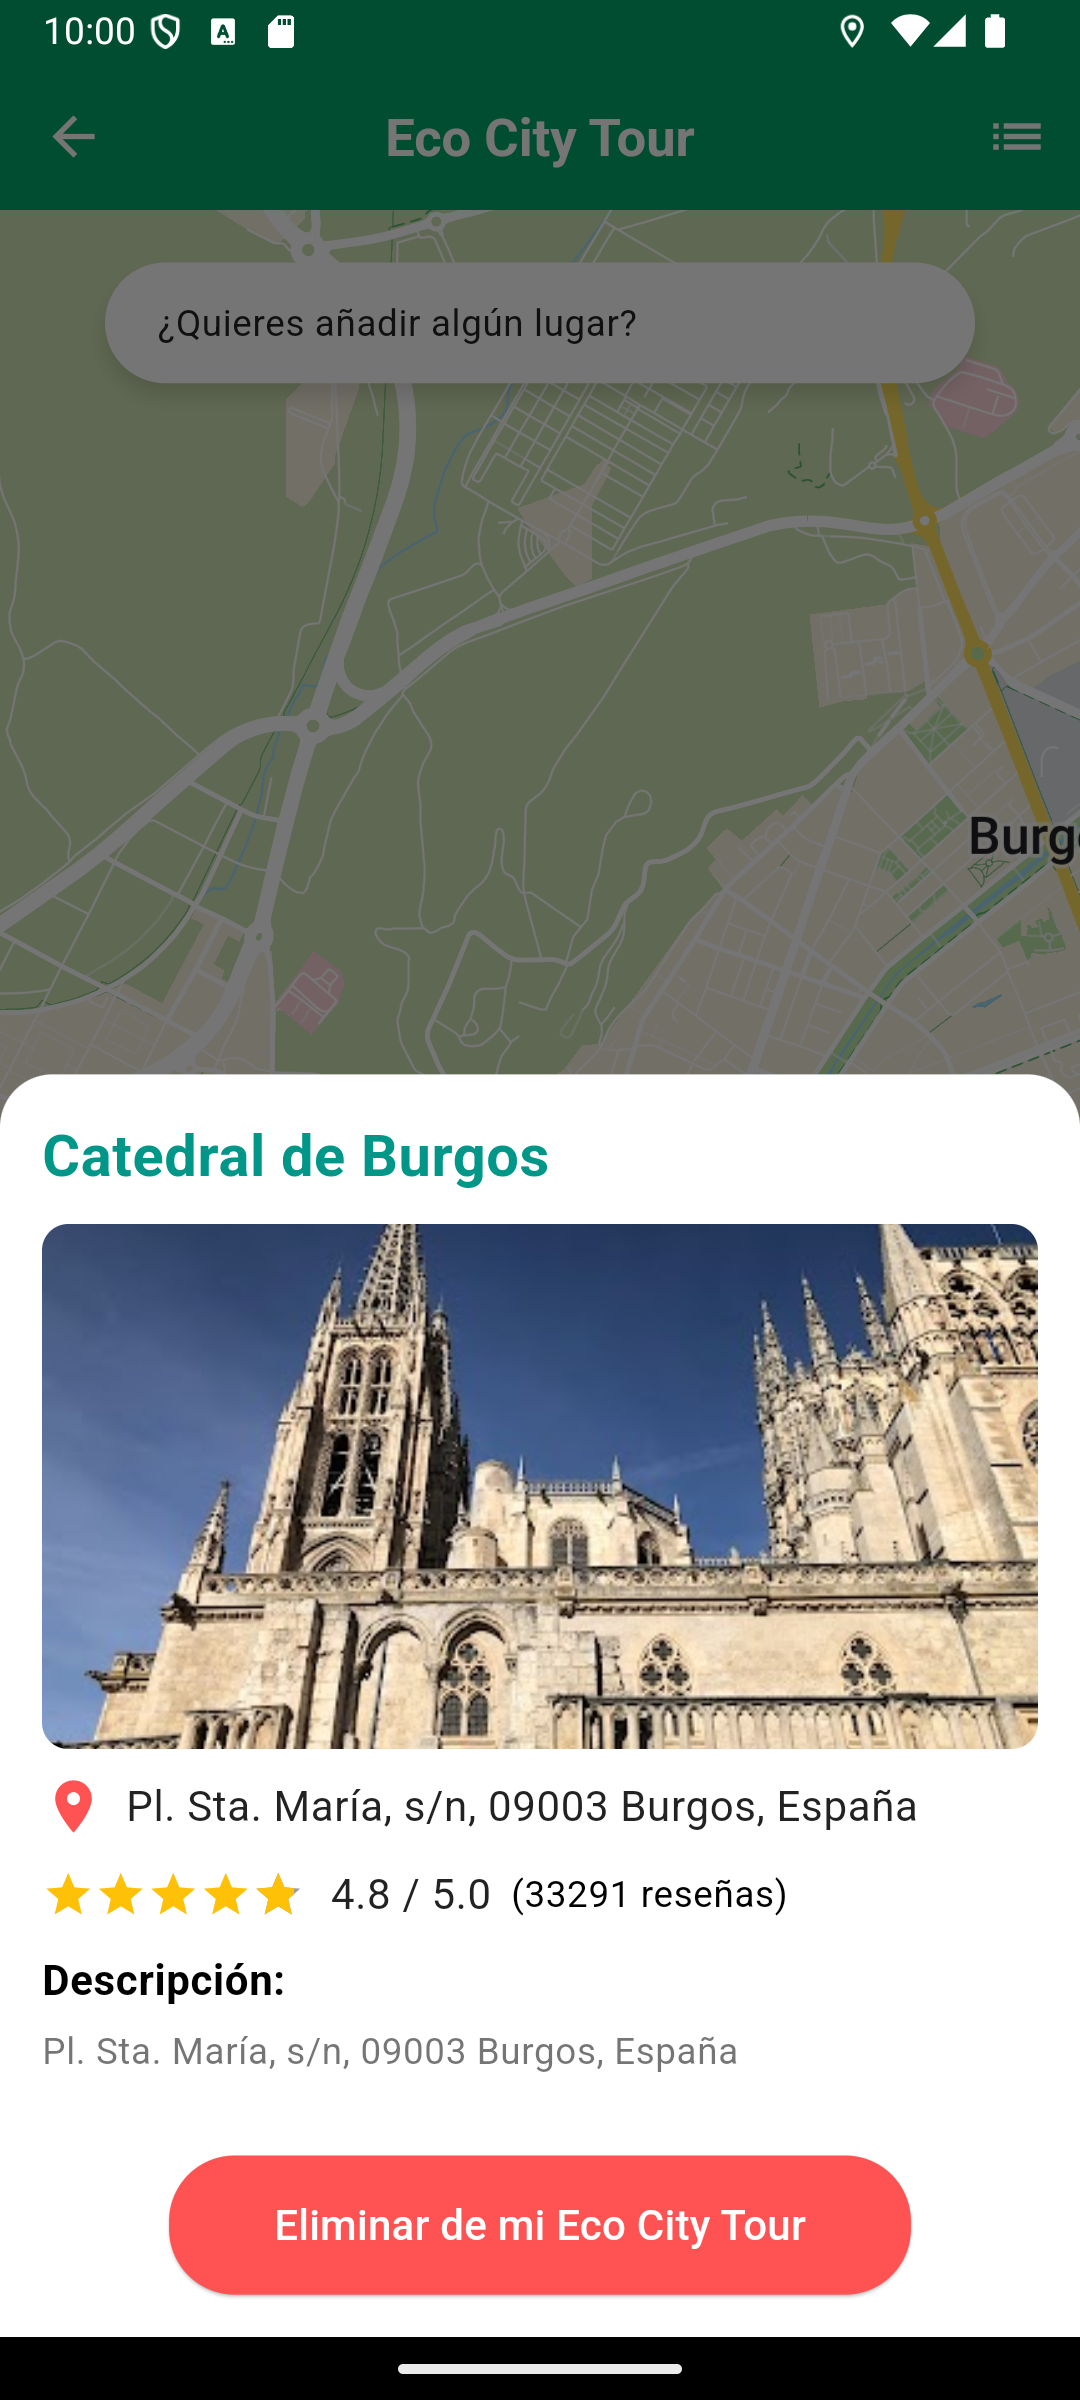
\includegraphics[width=0.6\linewidth]{E5-PDI-detalle} & 
		\vspace{-10pt}
		
		La primera acción que debe realizar el usuario al iniciar la aplicación es habilitar el permiso de uso de GPS. Esto permite que la aplicación acceda a la ubicación del dispositivo para calcular rutas y mostrar información relevante.
		\textbf{Pasos a seguir:}
		\begin{enumerate}
			\item Al abrir la aplicación por primera vez, aparecerá la pantalla mostrada en la Figura~\ref{fig:detallePDI}.
			\item Pulse el botón \textbf{Solicitar acceso al GPS}.
			\item Conceda el permiso solicitado en la ventana emergente.
		\end{enumerate}		
	\end{tabular}
	\caption{Detalle de \acrshort{pdi}}
	\label{fig:detallePDI}
\end{figure}

\subsection{Resumen de Eco City Tour creado}
\begin{figure}[h!]
	\centering
	\begin{tabular}{m{0.4\textwidth} m{0.55\textwidth}}
		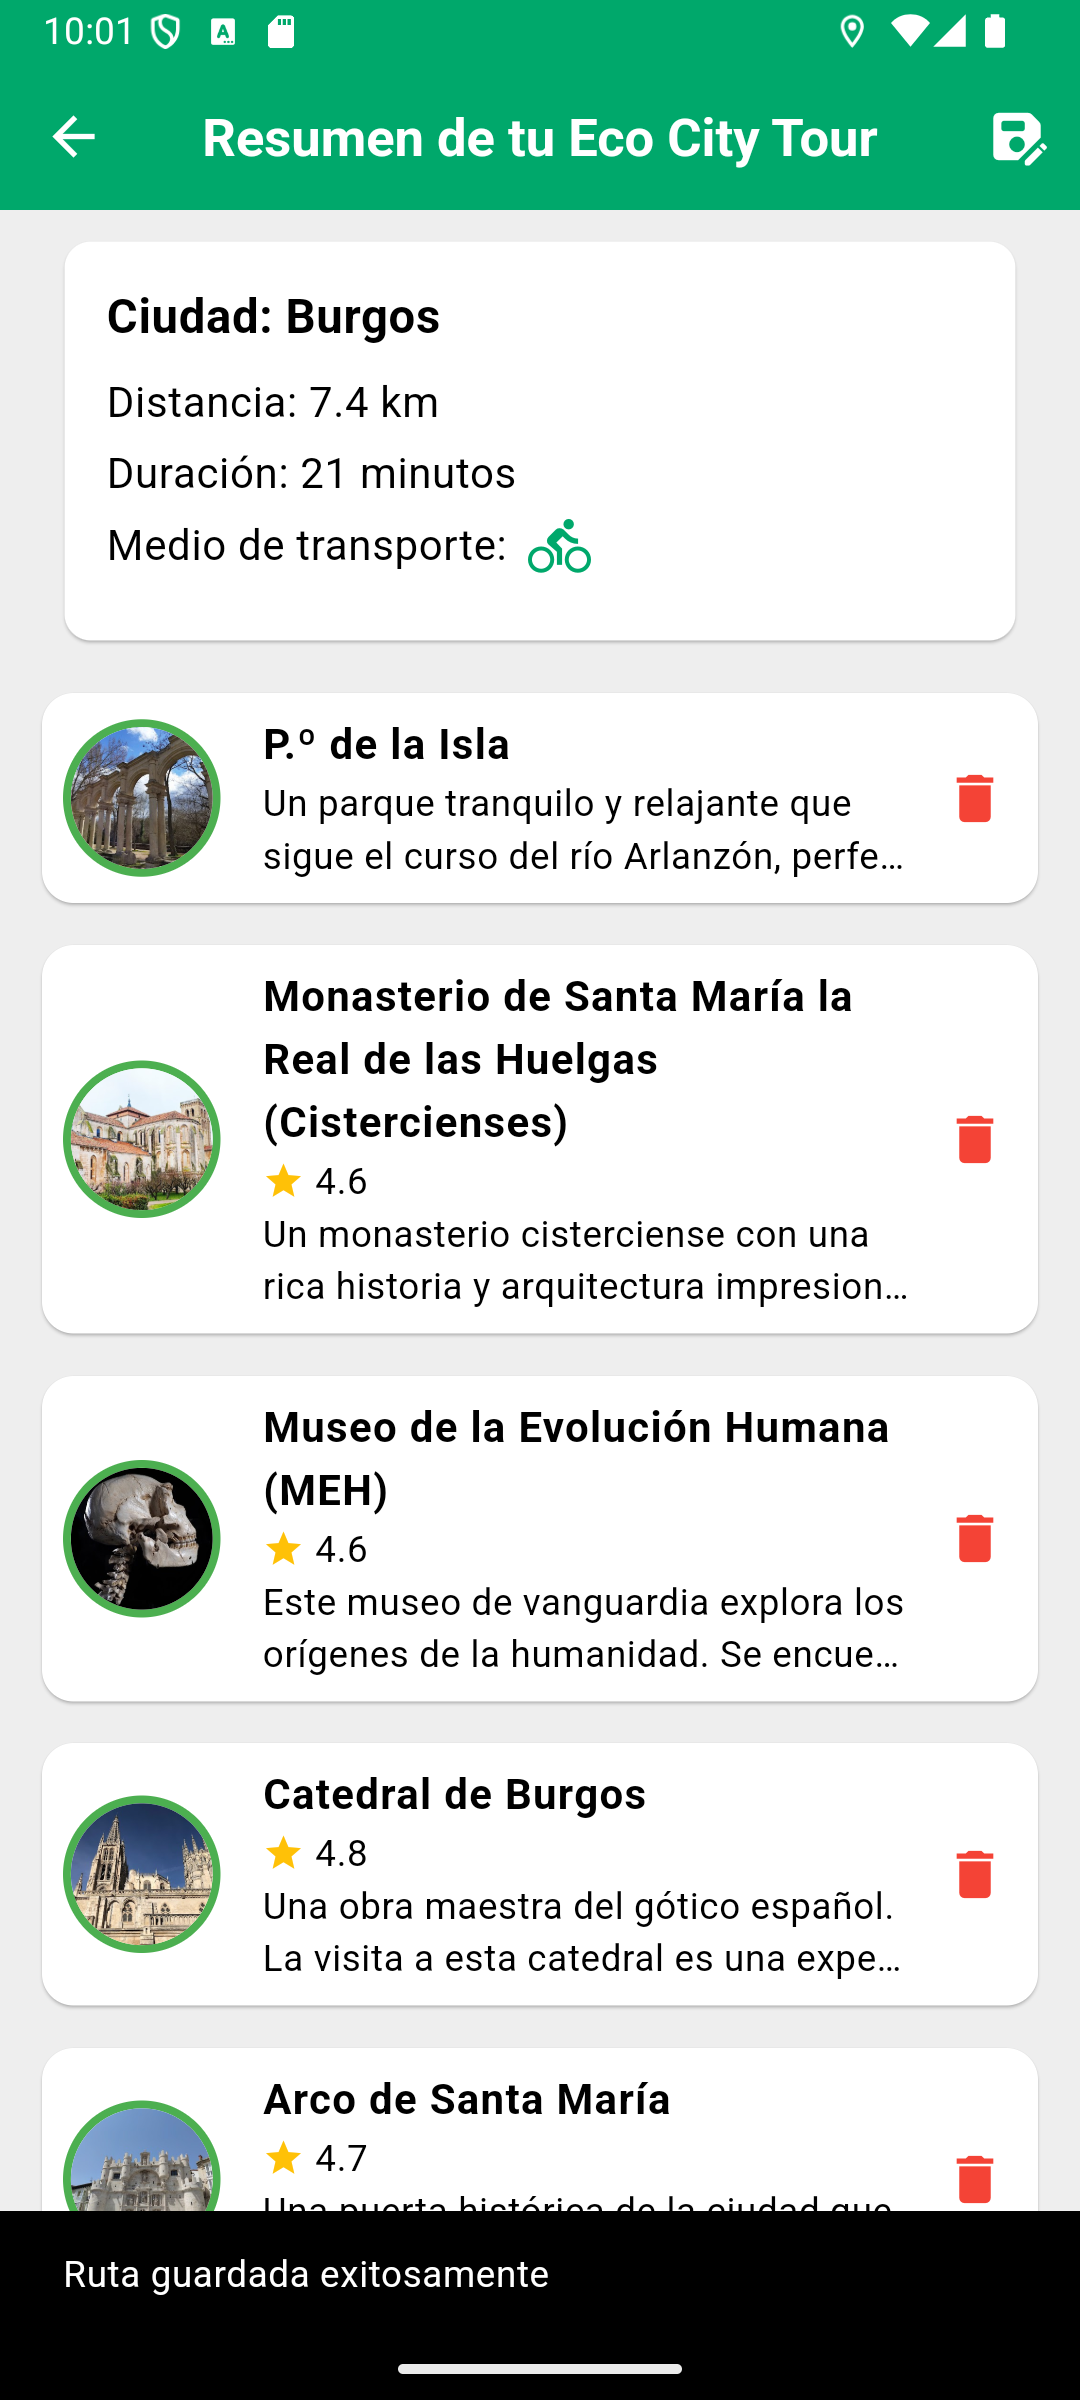
\includegraphics[width=0.6\linewidth]{E6-summary-screen} & 
		\vspace{-10pt}
		
		La primera acción que debe realizar el usuario al iniciar la aplicación es habilitar el permiso de uso de GPS. Esto permite que la aplicación acceda a la ubicación del dispositivo para calcular rutas y mostrar información relevante.
		\textbf{Pasos a seguir:}
		\begin{enumerate}
			\item Al abrir la aplicación por primera vez, aparecerá la pantalla mostrada en la Figura~\ref{fig:resumenECT}.
			\item Pulse el botón \textbf{Solicitar acceso al GPS}.
			\item Conceda el permiso solicitado en la ventana emergente.
		\end{enumerate}		
	\end{tabular}
	\caption{Pantalla de resumen del Eco City Tour}
	\label{fig:resumenECT}
\end{figure}

\subsection{Guardar Eco City Tour}
\begin{figure}[h!]
	\centering
	\begin{tabular}{m{0.4\textwidth} m{0.55\textwidth}}
		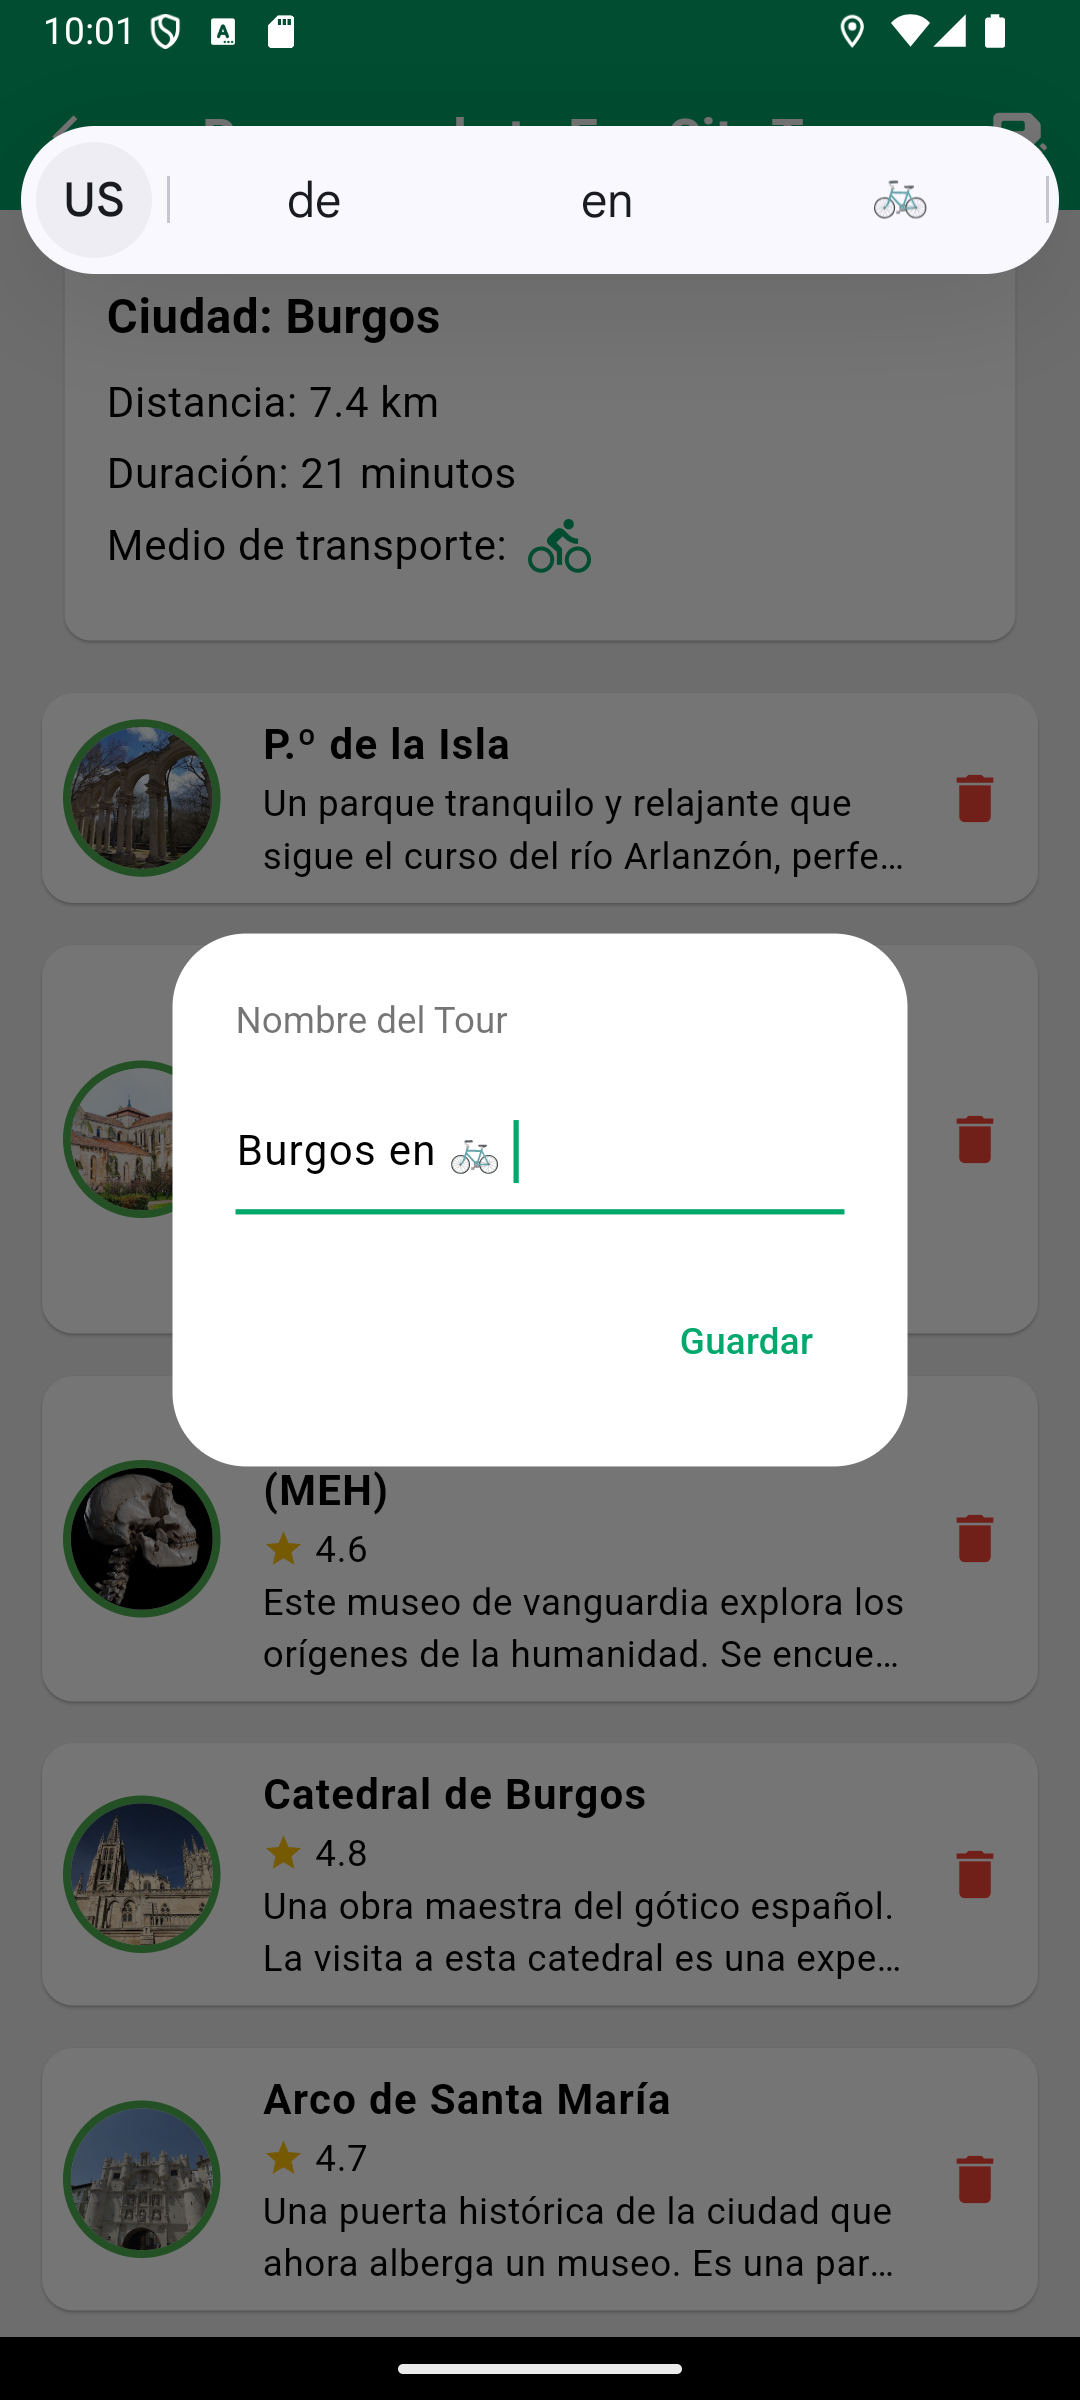
\includegraphics[width=0.6\linewidth]{E7-save-tour} & 
		\vspace{-10pt}
		
		La primera acción que debe realizar el usuario al iniciar la aplicación es habilitar el permiso de uso de GPS. Esto permite que la aplicación acceda a la ubicación del dispositivo para calcular rutas y mostrar información relevante.
		\textbf{Pasos a seguir:}
		\begin{enumerate}
			\item Al abrir la aplicación por primera vez, aparecerá la pantalla mostrada en la Figura~\ref{fig:saveECT}.
			\item Pulse el botón \textbf{Solicitar acceso al GPS}.
			\item Conceda el permiso solicitado en la ventana emergente.
		\end{enumerate}		
	\end{tabular}
	\caption{Pantalla de guardado del Eco City Tour}
	\label{fig:saveECT}
\end{figure}

\subsection{Cargar Eco City Tour}
\begin{figure}[h!]
	\centering
	\begin{tabular}{m{0.4\textwidth} m{0.55\textwidth}}
		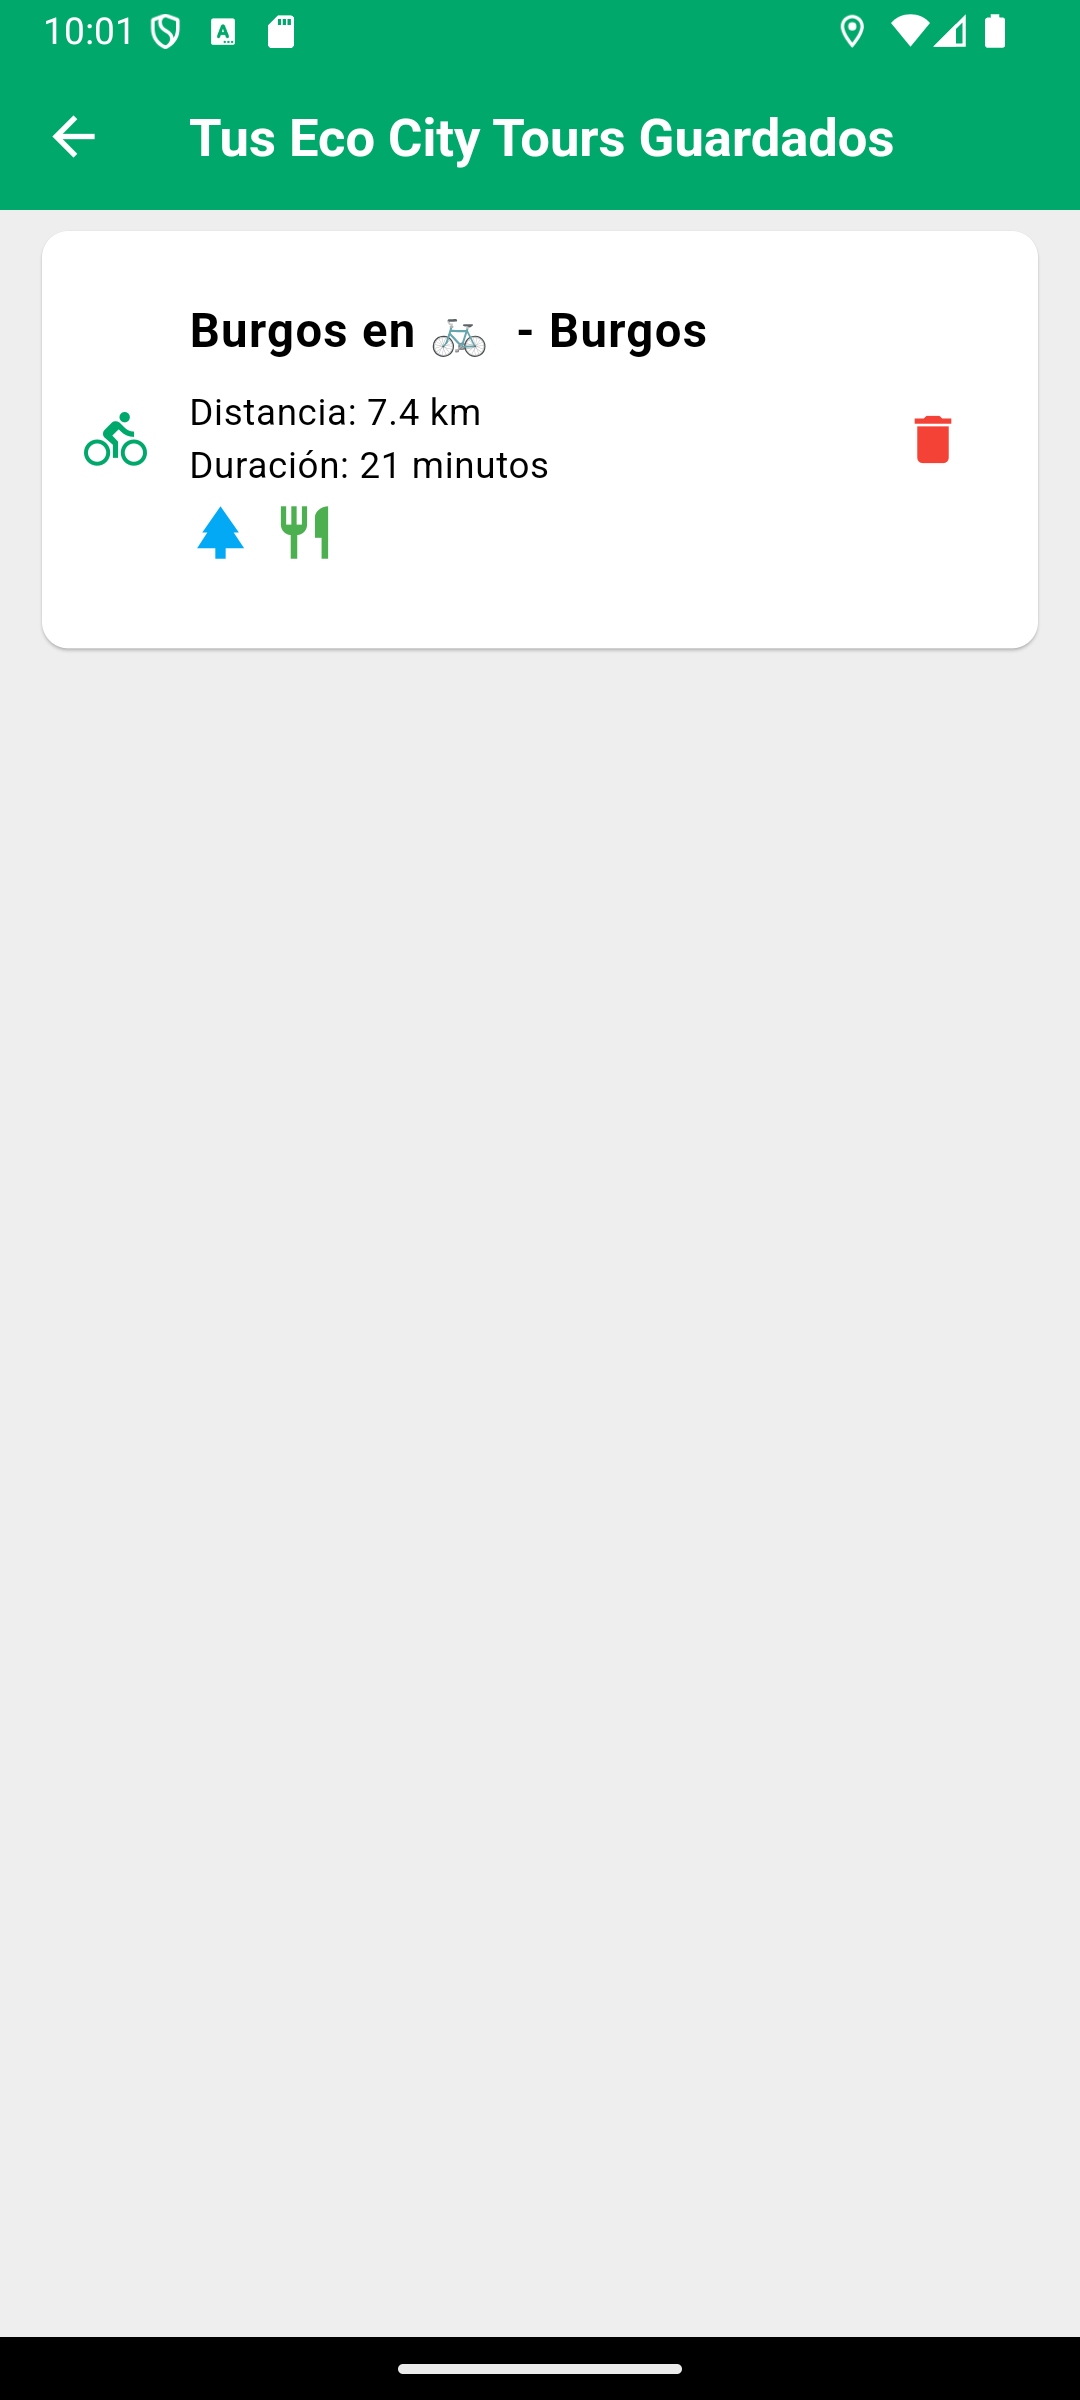
\includegraphics[width=0.6\linewidth]{E8-load-tour} & 
		\vspace{-10pt}
		
		La primera acción que debe realizar el usuario al iniciar la aplicación es habilitar el permiso de uso de GPS. Esto permite que la aplicación acceda a la ubicación del dispositivo para calcular rutas y mostrar información relevante.
		\textbf{Pasos a seguir:}
		\begin{enumerate}
			\item Al abrir la aplicación por primera vez, aparecerá la pantalla mostrada en la Figura~\ref{fig:loadECT}.
			\item Pulse el botón \textbf{Solicitar acceso al GPS}.
			\item Conceda el permiso solicitado en la ventana emergente.
		\end{enumerate}		
	\end{tabular}
	\caption{Pantalla de carga del Eco City Tour}
	\label{fig:loadECT}
\end{figure}

\subsection{Seguimiento en vivo de la posición del usuario}
\begin{figure}[h!]
	\centering
	\begin{tabular}{m{0.4\textwidth} m{0.55\textwidth}}
		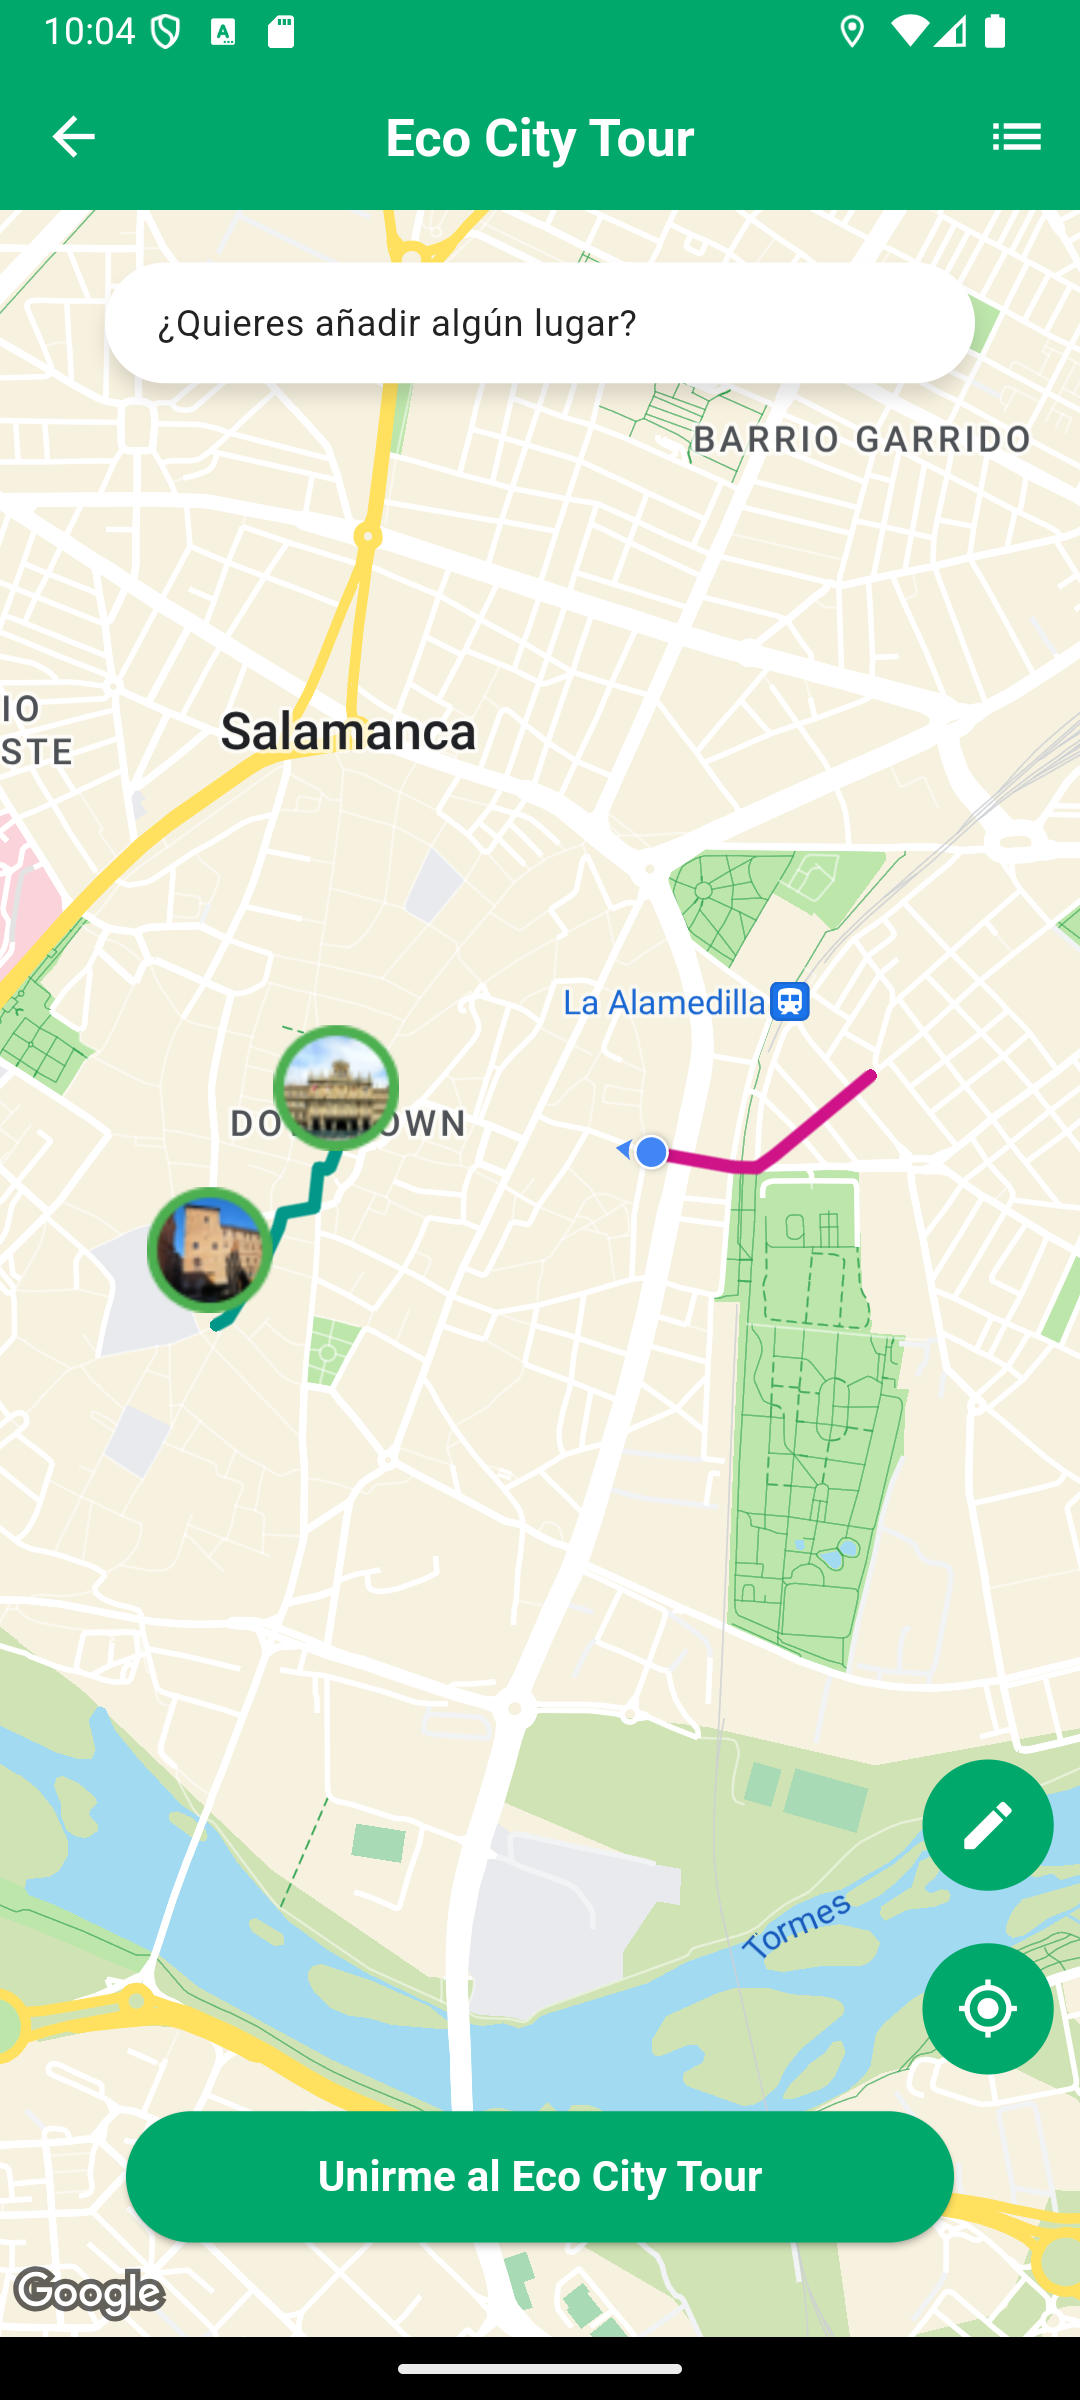
\includegraphics[width=0.6\linewidth]{E9-following-user} & 
		\vspace{-10pt}
		
		La primera acción que debe realizar el usuario al iniciar la aplicación es habilitar el permiso de uso de GPS. Esto permite que la aplicación acceda a la ubicación del dispositivo para calcular rutas y mostrar información relevante.
		\textbf{Pasos a seguir:}
		\begin{enumerate}
			\item Al abrir la aplicación por primera vez, aparecerá la pantalla mostrada en la Figura~\ref{fig:followingUser}.
			\item Pulse el botón \textbf{Solicitar acceso al GPS}.
			\item Conceda el permiso solicitado en la ventana emergente.
		\end{enumerate}		
	\end{tabular}
	\caption{Seguimiento en vivo de la posición del usuario}
	\label{fig:followingUser}
\end{figure}

\subsection{Unirse al Eco City Tour}
\begin{figure}[h!]
	\centering
	\begin{tabular}{m{0.4\textwidth} m{0.55\textwidth}}
		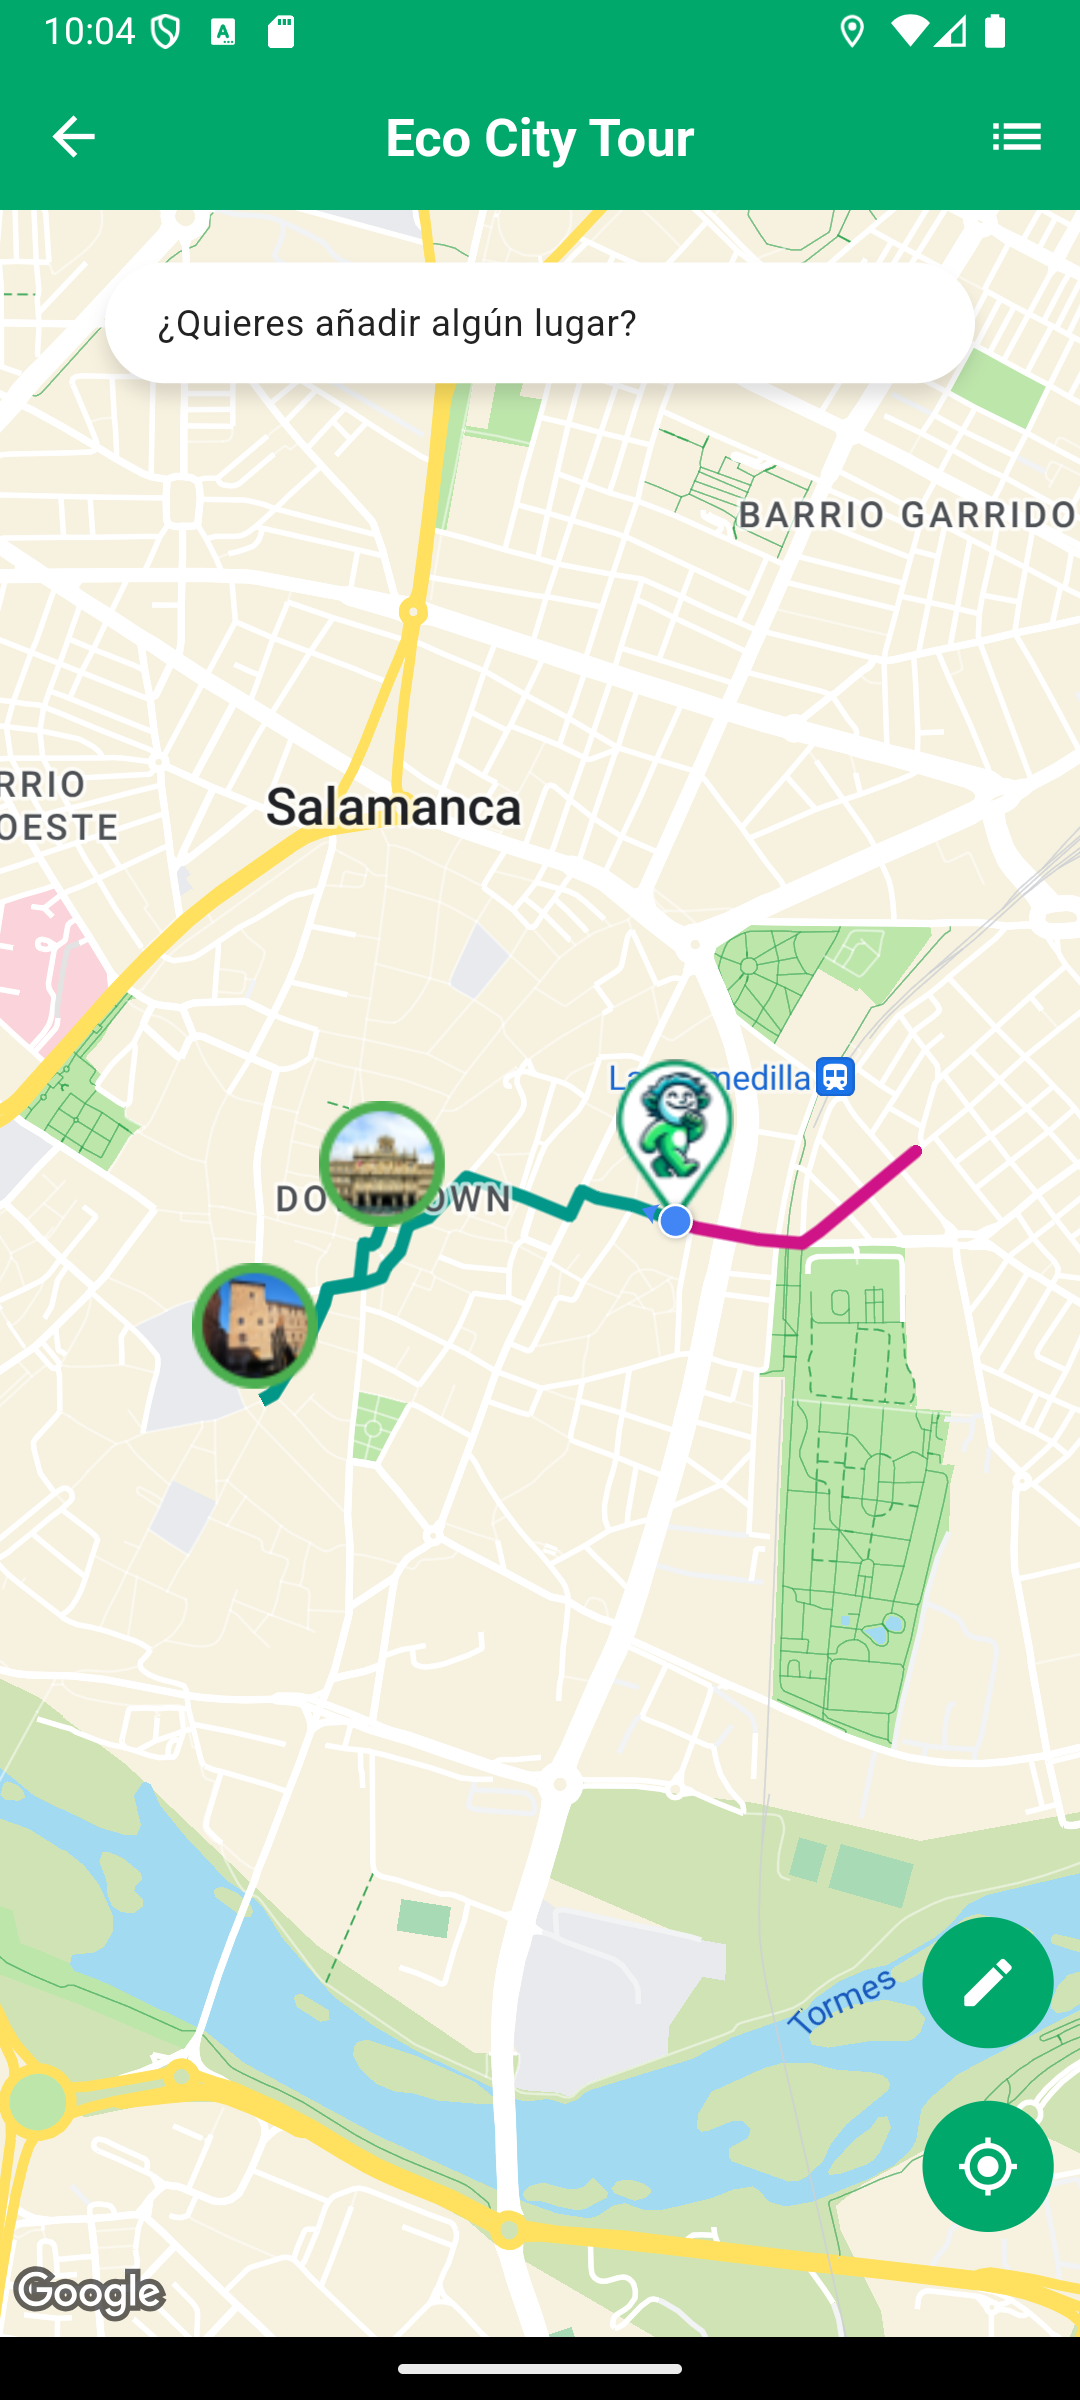
\includegraphics[width=0.6\linewidth]{E10-join-tour} & 
		\vspace{-10pt}
		
		La primera acción que debe realizar el usuario al iniciar la aplicación es habilitar el permiso de uso de GPS. Esto permite que la aplicación acceda a la ubicación del dispositivo para calcular rutas y mostrar información relevante.
		\textbf{Pasos a seguir:}
		\begin{enumerate}
			\item Al abrir la aplicación por primera vez, aparecerá la pantalla mostrada en la Figura~\ref{fig:joinECT}.
			\item Pulse el botón \textbf{Solicitar acceso al GPS}.
			\item Conceda el permiso solicitado en la ventana emergente.
		\end{enumerate}		
	\end{tabular}
	\caption{Unirse al Eco City Tour}
	\label{fig:joinECT}
\end{figure}
\apendice{Anexo de sostenibilización curricular}

\section{Introducción}
Este anexo incluirá una reflexión personal del alumnado sobre los aspectos de la sostenibilidad que se abordan en el trabajo.
Se pueden incluir tantas subsecciones como sean necesarias con la intención de explicar las competencias de sostenibilidad adquiridas durante el alumnado y aplicadas al Trabajo de Fin de Grado.

Más información en el documento de la CRUE \url{https://www.crue.org/wp-content/uploads/2020/02/Directrices_Sosteniblidad_Crue2012.pdf}.

Este anexo tendrá una extensión comprendida entre 600 y 800 palabras.



\bibliographystyle{plain}
\bibliography{bibliografiaAnexos}

\end{document}
